%%
%%  AaltoTheses - LaTeX-tutkielmapohjat Aalto-tyylille
%%
%%  Hau Phan
%%  hau.phan@aalto.fi
%%
\begin{filecontents*}{\jobname.xmpdata}
  \Title{Normalizing Flows for Graph Generation}
  \Author{Hannu Tiitu}
  \Keywords{graph neural network\sep normalizing flows\sep continuous normalizing flows\sep graphs generation\sep machine learning\sep geometric machine learning}
  \Publisher{Aalto University}
\end{filecontents*}
\documentclass[oneside,pdfa]{aaltoseries}
\makeatletter
\@ifpackageloaded{inputenc}{%
  \inputencoding{utf8}}{%
  \usepackage[utf8]{inputenc}}
\hypersetup{hidelinks}                % Linkkien korostus pois
\makeatother
\usepackage[finnish,english]{babel}   % Kieli on englanti, tiivistelmässä suomi
\usepackage{setspace}                 % Rivivälin säätämiseksi
\usepackage{afterpage}                % Sivun taustaväri
\microtypesetup{letterspace=25}       % Kannen harvaan välistykseen
\usepackage{lastpage}
\usepackage[round]{natbib}
\usepackage{amsmath}
\usepackage{amssymb}
\usepackage{bm}

\newtheorem{theorem}{Proposition}



\author{Hau Phan}
\title{Normalizing Flows for Graph Generation}

\begin{document}



%%  KANSI  ---------------------------------------------

\thispagestyle{empty}
\setcounter{page}{0}  % Kansisivulle sivunumero 0

% Kansisivun marginaalit
\newgeometry{left=23.2mm,right=23.2mm,top=13.5mm,bottom=18mm}

% Punainen kansisivu
\pagecolor{aaltoRed}\afterpage{\nopagecolor}
{\color{black}  % Musta teksti

	{\parindent0pt % Kappaleiden sisennys pois päältä
		{\fontsize{11.9pt}{11.9pt}\bfseries\sffamily\lsstyle Bachelor’s Programme in Science and Technology}

		\color{white}  % Valkoinen teksti alkaa

		\vspace{13.1mm}

		\begin{spacing}{3.1}
			{\fontsize{35}{35}\selectfont Normalizing Flows \\ for Graph Generation}
		\end{spacing}

		\vspace{2.2mm}

		\begin{spacing}{1.24}
			{\fontsize{14pt}{14pt}\bfseries\sffamily\lsstyle A Literature Review}
		\end{spacing}

		\vspace{7.2mm}

		\rule{\textwidth}{1.25pt}

		\vspace{8.5mm}

		{\fontsize{13.9pt}{13.9pt}\bfseries\sffamily\lsstyle Hau Phan}

		\vfill

		\begin{picture}(0,0)
			\put(356,-7.8){\bfseries\sffamily\footnotesize\lsstyle BACHELOR'S}
			\put(356,-17.4){\bfseries\sffamily\footnotesize\lsstyle THESIS}
			\put(346,-26.5){\rule{.75pt}{25pt}}
		\end{picture}

		\AaltoLogoSmall{.66}{?}{white}

	} % Kappaleiden sisennys takaisin käyttöön
} % Valkoisen tekstin pääätös



%%  NIMIÖSIVU  -----------------------------------------

\newpage

\pagenumbering{roman}

% Nimiösivun marginaalit
\newgeometry{left=80.7mm,right=25mm,top=12.9mm,bottom=21mm}

\thispagestyle{empty}

{\parindent0pt % Kappaleiden sisennys pois päältä
	\begin{spacing}{1.1}
		\hspace{-39.1mm}{\fontsize{10.5pt}{10.5pt}\sffamily\lsstyle Aalto University}

		\hspace{-39.1mm}{\fontsize{10.5pt}{10.5pt}\bfseries\sffamily\lsstyle BACHELOR'S THESIS} {\sffamily\lsstyle \the\year}
	\end{spacing}

	\vspace{12.7mm}

	\begin{spacing}{1.63}
		{\fontsize{17.8pt}{17.8pt}\selectfont Normalizing Flows \\for Graph Generation}
	\end{spacing}

	\vspace{10.5mm}

	\begin{spacing}{1.2}
		{\fontsize{13pt}{13pt}\selectfont A Literature Review}
	\end{spacing}

	\vspace{10.6mm}

	{\fontsize{13.9pt}{13.9pt}\bfseries\sffamily\lsstyle Hau Phan}

	\vfill

	{\fontsize{10.3pt}{10.3pt}\sffamily\lsstyle\raggedright
		\begin{spacing}{1.06}

			Thesis submitted in partial fulfillment of the requirements for the
			degree of Bachelor of Science in Technology.

			Otaniemi, September 9, 2022

			\begin{tabbing}
				Supervisor:\hspace{6mm} \= Maarit Käpylä \\
				Advisor: \> Anirudh Jain
			\end{tabbing}
			\vspace{-4mm}
		\end{spacing}
	} % fontsize

	\vspace{11.5mm}

	\begin{spacing}{.9}
		{\bfseries\sffamily\lsstyle Aalto University \\
			School of Science \\
			Bachelor’s Programme in Science and Technology}
	\end{spacing}
} % Kappaleiden sisennys takaisin käyttöön



%%  ABSTRACT  ------------------------------------------

\newpage
\phantomsection
\addcontentsline{toc}{chapter}{Abstract}

% Tiivistelmien marginaalit
\newgeometry{left=41.8mm,right=25mm,top=14.33mm,bottom=27mm}
% Alkuperäisessä Aalto-sarjassa marginaalit ovat suunnilleen näin:
%\newgeometry{left=41.8mm,right=17.6mm,top=14.33mm,bottom=20.4mm}

\begin{spacing}{.88}

	{\parindent0pt % Kappaleiden sisennys pois päältä
	\AaltoLogoSmall{.625}{''}{aaltoBlack}

	{\fontsize{13.9pt}{13.9pt}\selectfont
		\vspace{-8.9mm}\hfill{\bfseries\sffamily\lsstyle Abstract}}

	{\fontsize{9.48pt}{9.48pt}\selectfont
		\vspace{.9mm}\hfill{\bfseries\sffamily\lsstyle Aalto University, P.O. Box 11000, FI-00076 Aalto~~\textcolor{aaltoGray}{www.aalto.fi}}}

	\vspace{7.8mm}{\fontsize{10.5pt}{10.5pt}\bfseries\sffamily\lsstyle Author}\\
	{\small Hau Phan}

	\vspace{-2.4mm}\rule{\textwidth}{.75pt}

	{\fontsize{10.5pt}{10.5pt}\bfseries\sffamily\lsstyle Title}\\
	\parbox[t]{\textwidth}{\raggedright\small Normalizing Flows for Graph Generation}

	\vspace{.5mm}\rule{\textwidth}{.75pt}

	{\fontsize{10.5pt}{10.5pt}\bfseries\sffamily\lsstyle School}~~{\small School of Science}

	\vspace{-2.4mm}\rule{\textwidth}{.75pt}

	{\fontsize{10.5pt}{10.5pt}\bfseries\sffamily\lsstyle Degree programme}~~{\small Bachelor’s Programme in Science and Technology}

	\vspace{-2.4mm}\rule{\textwidth}{.75pt}

	{\fontsize{10.5pt}{10.5pt}\bfseries\sffamily\lsstyle Major}~~{\small Data Science }\hfill{\fontsize{10.5pt}{10.5pt}\bfseries\sffamily\lsstyle Code}~~{\small IL3011}

	\vspace{-2.4mm}\rule{\textwidth}{.75pt}

	{\fontsize{10.5pt}{10.5pt}\bfseries\sffamily\lsstyle Supervisor}~~{\small Maarit Käpylä}

	\vspace{-2.4mm}\rule{\textwidth}{.75pt}

	{\fontsize{10.5pt}{10.5pt}\bfseries\sffamily\lsstyle Advisor}~~{\small Anirudh Jain}

	\vspace{-2.4mm}\rule{\textwidth}{.75pt}

	{\fontsize{10.5pt}{10.5pt}\bfseries\sffamily\lsstyle Level}~~{\small
  Bachelor's thesis}\hfill{\fontsize{10.5pt}{10.5pt}\bfseries\sffamily\lsstyle
  Date}~~{\small September 9, 2022}\hfill{\fontsize{10.5pt}{10.5pt}\bfseries\sffamily\lsstyle Pages}~~{\small \pageref{LastPage}}\hfill{\fontsize{10.5pt}{10.5pt}\bfseries\sffamily\lsstyle Language}~~{\small English}

	\vspace{-2.4mm}\rule{\textwidth}{.75pt}

	\vspace{6mm}

	} % Kappaleiden sisennys takaisin käyttöön
\end{spacing}
\begin{spacing}{1.05}

	\noindent{\fontsize{10.5pt}{10.5pt}\bfseries\sffamily\lsstyle Abstract}
	\vspace{.8mm}

  {\small Deep learning (DL) has attracted significant research attention in
  recent years due to its effectiveness in capturing latent representations of
  Euclidean data, such as images, audio, and natural languages. However, not all
  data is Euclidean and there is a resurgence of applications of data
  represented as discrete structures such as graphs that expresses abstract
  relations between objects. One such relevant task on graphs is generative
  modeling where the objective is to model the discrete distribution of
  molecules, social networks, logistic chains and other realization of graphs
  given samples drawn from it. Such tasks are notoriously difficult due to
  various irregularity of graphs such as permutation invariance and
  discreteness, yet is renownedly rewarding due to its importance in drug
  discovery and property optimization. Generally, most difficulties can be
  attributed to the discrete nature of graphs, which incurs a significant needs
  for accurate deterministic density evaluation and sampling.

  Normalizing flows are novel generative models with the promise of producing
  tractable distributions while remains efficient and exact in their density
  estimation and sampling. Useful latent space representation is also a
  complimenting property for flows model, allowing interpolation and guided
  optimization to be easily performed. Due to these desirable properties,
  normalizing flows have experienced a resurgence in popularity in the past
  couple years, specifically in the domain of \textit{de novo} molecule
  generation.

  This thesis presents a systematic methodological exploration of normalizing
  flows with deliberate attentions to graph neural networks (GNNs), explored and
  categorized under a modified version of message passing. Moreover, this thesis
  also reviews contemporary literature and provide explanations and contexts for
  a diverse set of approaches to normalizing flows and GNNs individually.
  Exemplary works on state-of-the-arts flow-based models on molecules
  are also explored in detail formalism, classified and compared. As a result,
  such exploration ultimately 1) reveals various advantages and disadvantages of
  both autoregressive and one shot approach to generate graphs with flows, and
  2) identify future research paths for extending existing flow architectures.
	}

	\vfill

\end{spacing}
\begin{spacing}{.88}
	{\parindent0pt % Kappaleiden sisennys pois päältä

  \makebox[19mm][l]{\fontsize{10.5pt}{10.5pt}\bfseries\sffamily\lsstyle
  Keywords}\parbox[t]{123.6mm}{\raggedright\small graph neural network,
  normalizing flows, graph generation, molecule generation, generative modeling, density estimation}

	\vspace{.5mm}\rule{\textwidth}{.75pt}

	{\fontsize{10.5pt}{10.5pt}\bfseries\sffamily\lsstyle urn}~~{\small https://aaltodoc.aalto.fi}

	\vspace{-2.4mm}\rule{\textwidth}{.75pt}

	} % Kappaleiden sisennys takaisin käyttöön
\end{spacing}



%%  SISÄLTÖ  -------------------------------------------

\newpage

\tableofcontents

%%  TYÖ ALKAA TÄSTÄ  -----------------------------------

\newpage

\pagenumbering{arabic}

\chapter{Introduction}

\section{Motivation}

\subsubsection{Non-Euclidean data and graph}

Deep learning (DL) has attracted significant research attention in recent years
due to its effectiveness in capturing latent representations of Euclidean data,
such as images, audio, and natural languages. However, not all data is Euclidean
and there is a resurgence of applications of data represented as discrete
structures such as graphs, sets, and mappings that expresses abstract relations
between objects. In particular, graphs are among the most fundamental structures
in nature and can be observed everywhere across multiple domains. For example,
molecules are essentially graphs of atoms bonded to one another by chemical
bonds; users-products graphs are bipartite graphs that imply preferences of a
customer towards specific sets of products; citation networks represents
citationships between academic papers and inter/cross connections between
scientific domains; road networks and traffics flows can also be considered as
attributed spatial temporal graphs bestowed with directions. Graphs are
everywhere since they model connections and relationships, which are high-order
abstractions and thus ubiquitous in nature. However, graphs are also arbitrarily
complex mathematical objects: they can be irregular and have arbitrary numbers
of nodes and vertices, where nodes and edges can be numbers, vectors or even
smaller "child" graphs; they are also invariant with respect to rotation,
translation and permutation as there are no markers of direction or origin with
graphs \citep{bronsteinGeometricDeepLearning2017}. This is in direct contrast to
Euclidean data (e.g. images) where the notion of directions and rotations is
straightforward to define. The complexity that accompanies the expressive power
of graphs has posed significant challenges to existing deep learning methods
that were once successfully applied on Euclidean data. For example, the
convolution operation of convolution neural network (CNN), which is
straightforward to define for images but is non trivial for graphs due to their
permutation invariant property \citep{wuComprehensiveSurveyGraph2021}. The
domain of performing machine learning on graphs was summarized by the
encompassing term \textit{graph representation learning} which consists of
various deep learning and non-deep-learning approaches to learn latent
representations of graphs. Overall, devising new approaches to bridge the gap
between deep learning on Euclidean and non-Euclidean data has been a popular
topic recently among machine learning (ML) researchers.

\subsubsection{Generative modeling}

An interesting subdomain of machine learning is generative modeling which aims
to generate new data/observation that is similar (in some abstract
representation) to other samples seen in a given dataset. Most generative
methods usually consist of an \textit{inference} phase that learns a latent
distribution of the data and a \textit{sampling} phase that samples from it
using various methods. Generative modeling in particular has been popularized to
various modalities since the introduction of Generative Adversarial Network
(GANs) \citep{goodfellowGenerativeAdversarialNetworks2014} and Variational
Autoencoder (VAEs) \citep{kingmaAutoEncodingVariationalBayes2014}, where both had
shown remarkable success in generating new images of faces, scenery and even
audio \citep{hersheyCNNArchitecturesLargescale2017}. For graphs generation in
particular, the majority of research efforts are directed at solving the
molecular graph generation problem, which have high practical value in drug
discovery \citep{wuComprehensiveSurveyGraph2021}.

Generally speaking, there are
two primary approaches to generate new molecular graphs that are actively
explored: \textit{sequential generation} and \textit{global generation}.
Sequential approaches generate graphs by proposing nodes and edges step by step,
while global approaches output new graphs all at once, which is also referred to as
\textit{one-shot generation}. Pioneers in generating graph sequentially include
graph generation using SMILE representation
\citep{kusnerGrammarVariationalAutoencoder2017,
gomez-bombarelliAutomaticChemicalDesign2018}, DeepGMG
\citep{liLearningDeepGenerative2018} and GraphRNN
\citep{youGraphRNNGeneratingRealistic2018}. For global approaches, existing deep
learning architectures based on GANs and VAEs are adapted to graph domain by
replacing CNN layers with Graph Neural Network (GNN) layers, albeit, with certain differences in
architectural choices. Notable works from this line of research include MolGAN
\citep{decaoMolGANImplicitGenerative2018}, GraphVAE
\citep{simonovskyGraphVAEGenerationSmall2018} and NetGAN
\citep{bojchevskiNetGANGeneratingGraphs2018}.

An exciting path of research in generative modeling is to adapt
\textit{normalizing flows} to graph domain, which has experienced a surge in
popularity due to various desirable properties of flow-based models such as
exact and tractable likelihood, efficient sampling and usable latent space for
downstream tasks. Broadly speaking, the normalizing flows framework aims to
learn a continuous invertible and deterministic mapping between the data
distribution and the latent distribution, which is usually a Gaussian
distribution. Sampling can be conducted by sampling from the latent distribution
and passing through the reverse mapping to retrieve a sample from the data
distribution. The mappings here are simply continuous invertible functions or
compositions of them. Designing functions that are computationally efficient to
compose these mappings is the main focus when improving the expressivity of
these models \citep{kobyzevNormalizingFlowsIntroduction2021}. Notable works in
applying normalizing flows to graphs include GraphNVP
\citep{madhawaGraphNVPInvertibleFlow2019}, GraphAF
\citep{shiGraphAFFlowbasedAutoregressive2020} and MoFlow
\citep{zangMoFlowInvertibleFlow2020}. A recent novel development in normalizing
flows models are \textit{continuous flows}, where rather than a discrete
sequence of transformations that are chained together, the invertible mapping is
modeled as a solution to an ordinary differential equation (ODE). Continuous
time-dependent mappings allow the data distribution to smoothly "morphed" into
the latent distribution, although in practice, demand slightly more computation
due to additional queries of black-box ODE solvers. One of the most notable
works in the domain of continuous flow is FFJORD
\citep{grathwohlFFJORDFreeformContinuous2018} which is a direct followup
improvement of the popular work on Neural ODEs (NODE)
\citep{chenNeuralOrdinaryDifferential2019} that first formulated residual
networks and normalizing flows as continuous differential processes. Practical
applications of continuous flows, however, is a sparsely explored domain. This
thesis aims to provide a systematic depth-wise exploration of normalizing flow
models for graph generation, with focus on GNNs as the primary computational
building blocks for flows and molecule generation as the targeted task.

\section{Thesis outline}

The remaining of the thesis consists of four sections, starting with Section
\ref{c:nf}, where an exploration of normalizing flows including motivation,
formulation, and categorization is introduced. Section \ref{c:gnn} primarily
focuses on topics of GNNs, explored under the \textit{Message Passing Framework}
\citep{gilmerNeuralMessagePassing2017}, however, compressed and filtered in
terms of relevance to graph normalizing flows. Lastly, Section \ref{c:gnf}
consists of different applications of normalizing flows on graph data, with a
particular emphasis on molecule generation due to its high practical values and
being extensively studied. As for closing remarks, Section \ref{c:conclude}
gives a general concluding summary, limitations and a discussion on future paths
of graph generative models with normalizing flows.

\section{Notations}
This thesis adopts the convention of lowercase bold letters
($\mathbf{x,y,z}\ldots$) for vectors, uppercase bold letters
($\mathbf{A,E,V,W, H}\ldots$) for matrices and regular lowercase letters
($x,y,z$\ldots)
for scalar variables. However, there are some exceptions, which is either
explicitly stated in the surrounding context or listed below in the full notation table.
\begin{align*}
  \mathbb{R}^D &: \text{$D$-dimensional real-valued vector space} \\
  \mathbb{R}^{N \times N} &: \text{$N \times N$ real-valued matrix space} \\
  \mathbf{Y, Z} &: \text{Multivariate random variables (data/base
  distribution)} \\ p_{\mathbf{Y}}, p_{\mathbf{Z}} &: \text{Data/base
  distribution} \\ \mathbf{y, z} &: \text{A sample from the data/base
  distribution} \\ \mathbf{f, g}, F &: \text{Multivariate functions
  (normalizer/generator/generic function)} \\
  \mathbf{s}, \mathbf{t}, \mathbf{h} &: \text{Scale/translation/coupling function}\\
  \frac{\partial \mathbf{g}}{\partial \mathbf{x}} &:
  \text{Jacobian of $\mathbf{g}(\mathbf{x})$} \\ det \frac{\partial
  \mathbf{g}}{\partial \mathbf{x}} &: \text{Determinant of the Jacobian of
  $\mathbf{g}(\mathbf{x})$} \\ \mathbf{f} \circ \mathbf{g} &: \text{Composition
  of two functions $\mathbf{f}$ and $\mathbf{g}$} \\ \mathcal{N}(\mathbf{x};
  \mathbf{\mu}, \Sigma) &: \text{Multivariate normal distribution (mean
  $\mathbf{\mu}$ and covariance matrix $\Sigma$)} \\ U[0, 1]^{N} &:
  \text{Multivariate uniform distribution on $[0,1]^{N}$} \\ O(D), O(D^2) &:
  \text{Big-$O$ notations for algorithmic complexity} \\ \sigma (\cdot) &:
  \text{Sigmoid function} \\
  \text{ReLU}(\cdot), \text{Agg}(\cdot) &: \text{Explicit named functions/operations} \\
  \mathcal{G} = (\mathcal{V, E}, \mathbf{V, E}) &:
  \text{Graph with node set $\mathcal{V}$, edge set $\mathcal{E}$, node features
  $\mathbf{V}$ and edge features $\mathbf{E}$} \\
  N(v) &: \text{Neighborhood set of vertex $v$} \\
  [\mathbf{x}\,||\, \mathbf{y}] &: \text{Concatenation of two vectors} \\
  \mathfrak{F}, \mathfrak{F}^{-1} &: \text{Fourier transform, inverse Fourier transform}\\
\end{align*}
For tensor $\mathbf{E} \in \mathbb{R}^{N \times M \times K}$, the following
indexing notation is used:
\begin{align*}
  \mathbf{E}_{[i,j,k]} &: \text{Tensor entry of $\mathbf{E}$ at coordinate $(i,j,k)$} \\
  \mathbf{E}_{[i,:,:]} &: \text{$i$-th tensor slice in the first dimension} \\
  \mathbf{E}_{[i^-,:,:]} &: \text{Tensor slice without the $i$-th row in the
  first dimension} \\
  \mathbf{E}_{[<i,:,:]} &: \text{Tensor slice with index
  smaller than $i$ in the first dimension}
\end{align*}

\chapter{Normalizing Flows}
\label{c:nf}

One of the most straightforward to define but difficult to solve problems in
statistics is modeling a \textit{probability distribution} given samples drawn
from it. Broadly speaking, a probability distribution is a mathematical object
that assigns the \textit{chance} of some event occurring to some number. Formally, a
probability distribution is a \textit{measure} $\mu$ on a topological
\textit{sample space} $(\mathcal{X}, \sigma, \mu)$ mapping that space to the
interval $[0,1]$. Regardless of the choice of definition, modeling a probability
distribution can be reduced to searching some mappings or patterns on the data
space (albeit, with additional constraints imposed by probability axioms)
. This can be seen as an example of \textit{unsupervised learning} or
\textit{generative modeling}, which had accumulated great attention among
academics and the public alike. Its importance can be attributed to the
abundance of unlabeled data compared to labeled in nature, where it remains an
untapped source of information in training machine learning models. Moreover,
learning patterns in data is a high-level general capability that can be
utilized in practically every domain of science, from humanities such as
psychology to STEM fields such as physics. Common uses of generative
modeling in science include probability density estimation, dataset
summarization, outlier detection, and prior reconstruction, to name a few.

There have been various approaches in tackling this distribution modeling
problem. Direct analytic approaches based on the assumption that observations
were drawn from a fixed regular family of named distributions with parameters
that can be inferred. However, this is an extremely optimistic and restricting
assumption that might not be accurate for more complex multidimensional domains
in nature such as images and sound. Variational inference (VI) and expectation
maximization (EM) algorithms rely on latent variables to explain the data, but
also introduce further complexity during learning and inference. With the boom
of parallel computing architecture such as GPUs, novel deep learning approaches
were now viable for learning massive datasets in generative modeling, which was
exampled by the massive increase in numbers of publications on generative
adversarial networks (GANs) and variational autoencoders (VAEs). While these DL
architectures had shown impressive results in image generation tasks, there are
notable downsides of these black-box models. First is the inaccessible
probability density for new observations, which make it unsuitable for density
estimation tasks. Second is their notoriously difficult training and convergence
when implemented. Adversarial approaches are based on training competing models
that are uncertain to either converge to the true optimal or even converge at
all. Mode collapse/posterior collapses are frequent occurrences while training
GANs, which happens when the model learns a simplified distribution that covers
only some signature modes rather than a diverse set of them. Furthermore,
vanishing gradients are pervasive in DL models, since fundamentally, neural
models are composite functions: the longer the computation chain, the more
magnified errors and digression of gradients at output. Therefore, careful
monitoring regimes and various stabilizing mechanism, usually developed through
trial and errors, are employed when training these models.

Normalizing flow models is a novel family of generative models that are capable
of learning irregular complex distribution with exact density evaluation, while
also allowing efficient sampling. There have been numerous applications of
normalizing flows and approaches to improve on it being explored in the last
decade, spanning multiple scientific domains. Notable mentions include noise
modeling, audio generation, reinforcement learning, computer graphics and
physics simulation. For this thesis, application of normalizing flow for
molecular and graph generations are explored. Furthermore, for
conciseness, this thesis only investigates normalizing flows approaches that are
relevant to these applications in particular.

\section{Background}

A normalizing flow, as seen from a generation perspective, is a transformation
of a simple probability distribution (e.g. normal distribution) into a more
complex data distribution by a sequence of invertible and differentiable
mappings. During generation, a sample is drawn from the simple distribution and
undergoes the deterministic transformation to yield an output. For density
estimation, however, a slightly more complex procedure is performed: the
observation is first transformed by an inverse mapping associated with the
original transformation. Then the probability density of this observation (i.e.
the likelihood) can be accurately calculated by multiplying 1) the
probability density of the inverse-transformed sample under the simple
distribution, and 2) the corresponding change in volume associated by the chain of
inverse transformation. The change in volume is the product of the absolute
values of the determinants of the Jacobians for each transformation, as required
by the change of variables formula.

Normalizing flows hence can be seen as a systematic approach to model complex
distribution by first choosing a (simple) base distribution and chaining
together a sequence of differentiable, reversible, parameterized
transformations. Under this framework, the simple distribution is used as an
interface for sampling, likelihood estimation and interpolation which was
otherwise impossible to be done directly on the complex data distribution.

\subsection{Formal Definition}

Denote $\mathbf{Z} \in \mathbb{R}^D$ as the random variable following a
initially known tractable multivariate distribution with $p_{\mathbf{Z}}:
\mathbb{R}^D \to [0,1]$ as its probability density function. Similarly, let
$\mathbf{Y} \in \mathbb{R}^D$ with $p_{\mathbf{Y}}: \mathbb{R}^D \to [0,1]$. Let
also denote $\mathbf{g}$ an invertible function such that $\mathbf{Y} =
\mathbf{g}(\mathbf{Z})$. Denote its inverse as $\mathbf{f} = \mathbf{g}^{-1}$.
Then according to the change of variables equation, we have:
\begin{align}
  p_{\mathbf{Y}}(\mathbf{y}) &= p_{\mathbf{Z}}(\mathbf{f}(\mathbf{y})) \left|det
  \frac{\partial \mathbf{f}}{\partial \mathbf{y} } \right| \\
  p_{\mathbf{Z}}(\mathbf{z}) &= p_{\mathbf{Y}}(\mathbf{g}(\mathbf{z})) \left|det
  \frac{\partial \mathbf{g}}{\partial \mathbf{z} } \right|
\end{align}

Here $\frac{\partial \mathbf{f}}{\partial \mathbf{y} }$ and $\frac{\partial
\mathbf{g}}{\partial \mathbf{z}}$ denotes the Jacobians of $\mathbf{f}$ and
$\mathbf{g}$ respectively.

The above equations represent two directions of a normalizing flow:
the \textit{generative direction} where the base
distribution $p_{\mathbf{Z}}$ (also known as the 'noise') is \textit{push forward} to a more complex probability
distribution $p_{\mathbf{Y}}$ as indicated by the first equation; and the \textit{normalizing
direction} where the complex distribution $p_{\mathbf{Y}}$ is \textit{normalized} or
\textit{simplified} to the base distribution $p_{\mathbf{Z}}$. The function $\mathbf{g}$ is
aptly named the \textit{generator} while the function $\mathbf{f}$ is
referred to as the \textit{normalizer}. The terms normalizing flows is doubly
correct if the base distribution is chosen to be the normal distribution,
which is often the case in practice.

More formally, one can explain normalizing flow using the language of measure
theory, characterizing distributions as generic measurable spaces and the
functions $\mathbf{g}$ and $\mathbf{f}$ as diffeomorphisms between such spaces.
Such characterization is necessary for theoretical study of generative models on
non-Euclidean/discrete spaces and (Riemann) manifolds. This abstract perspective
on normalizing flow resonates with the works on optimal transportation theory
\citep{villaniTopicsOptimalTransportation2003}.

As noted by \citep{kobyzevNormalizingFlowsIntroduction2021}, it is worth
mentioning that commonly in the literature, diffeomorphisms are simply referred
to as "bijections" even though this naming is mathematically incorrect.
Generally speaking, it is not required that the pushforward function
$\mathbf{g}$ is differentiable everywhere, but rather differentiable "almost
everywhere with respect to the Lebesgue measure on $\mathbb{R}^D$"
\cite{kobyzevNormalizingFlowsIntroduction2021}. This allows
for \textit{piecewise differentiable functions} such as splines to be used in
the construction.

For inference (i.e., training the model) in practice, one simply maximize the
(log) likelihood of the training data as the objective and updates the flows
parameters with gradient ascend. Assuming the normalizer $\mathbf{f}_{\bm{\theta}}$ is
parameterized by some optimizable variables $\bm{\theta}$, and
independent training data
$(\mathbf{y}_i)_{i=1}^M$, then the log likelihood per sample can be written as:
$$
 \log p_{\mathbf{Y}}(\mathbf{y}_i) = \log p_{\mathbf{Z}}(\mathbf{f}(\mathbf{y}_i))
  + \log \left|det
  \frac{\partial \mathbf{f}}{\partial \mathbf{y}_i} \right|
.$$
And thus the objective is:
$$
\max_{\bm{\theta}} \log \prod_{i=1}^M p_{\mathbf{Y}}(\mathbf{y}_i) =
\max_{\bm{\theta}} \sum_{i=1}^{M}\log p_{\mathbf{Z}}(\mathbf{f}_{\bm{\theta}}(\mathbf{y}_i))
  +  \sum_{i=1}^{M} \log \left|det
  \frac{\partial \mathbf{f}_{\bm{\theta}}}{\partial \mathbf{y}_i} \right|
.$$

\subsection{Universality}
\label{f:uni}

Intuitively, given a complex enough generator $\mathbf{g}$, one can transform
any base distribution to a complex distribution under some reasonable
assumptions. In fact, the existence of such transformation has been proven
formally in the excellent treatment of normalizing flow by
\citep{papamakariosNormalizingFlowsProbabilistic2021}. A broad summary of the
proof is that by modeling $\mathbf{g}$ as an elementwise cumulative density
function (CDF) of the autoregressive conditional probabilities (assuming these
conditional probabilities are differentiable), it can be shown that arbitrary
complex distribution $p_{\mathbf{Y}}(\mathbf{y})$ can be transformed into a
uniform distribution on the open unit cube $(0,1)^D$ and such transform is
diffeomorphic by the monotonicity of CDF(s). The remaining part is to construct
a diffeomorphism from $(0,1)^D$ to the base distribution $p_{\mathbf{Z}}$, which
is trivial. Note that while such theoretical guarantees are useful, they might
not translate in practical settings since expressivity might be limited by other
architectural decisions in favor of efficiency.

\subsection{Composability}
\label{f:comp}

Although the requirement of diffeomorphic transformation is indeed a hard
constraint on the hypothesis space of possible architectures, it still permits the
ability to construct more complex transformations by composing
simpler flows. This is due to the mathematical fact that $(\mathcal{D}, \circ)$
(where $\mathcal{D}$ is
the set of all possible diffeomorphism on $\mathbb{R}^D$ and $\circ$ is
composition operator) forms a \textit{group} in $\mathbb{R}^D$, i.e., the set of
diffeomorphisms is \textit{closed} under composition. For example, one can
construct a complex normalizer $\mathbf{f}$ (and, likewise, $\mathbf{g}$) by composing a sequence of
$K$ diffeomorphism $(\mathbf{f}_i(\cdot))_{i=1}^K$:
$$
\mathbf{z} = \mathbf{f}(\mathbf{y}) = \mathbf{f}_K \circ \mathbf{f}_{K-1} \circ \ldots \circ \mathbf{f}_1
(\mathbf{y})
.$$
and the resulting function remains a diffeomorphism.

Furthermore, it is also possible to characterize $\mathbf{f}$ as a
\textit{multi-step process} that consists of multiple transformation stages.
Defines the intermediate states as $\mathbf{x}_0 = \mathbf{y}$, $\mathbf{x}_K =
\mathbf{z}$ $\mathbf{x}_i = \mathbf{f}(\mathbf{x}_{i-1})$ for $i=1,2, \ldots,
K$. Then the normalizing flow process induced by $\mathbf{f}$ and it inverse can
be written as

$$
\mathbf{y}
\underset{\mathbf{f}^{-1}_1}{\overset{\mathbf{f}_1}{\longleftrightarrow}}
\mathbf{x}_1
\underset{\mathbf{f}^{-1}_2}{\overset{\mathbf{f}_2}{\longleftrightarrow}}
\mathbf{x}_2 \ldots
\underset{\mathbf{f}^{-1}_K}{\overset{\mathbf{f}_K}{\longleftrightarrow}}
\mathbf{z}
.$$

By the chain rules, the change of variable equations become:
\begin{align}
  p_{\mathbf{Y}}(\mathbf{y}) &= p_{\mathbf{Z}}(\mathbf{z}) \prod_{i=1}^K \left|det
   \frac{\partial \mathbf{x}_i}{\partial \mathbf{x}_{i-1} } \right| \\
\implies
  \log p_{\mathbf{Y}}(\mathbf{y}) &= \log p_{\mathbf{Z}}(\mathbf{z}) +  \sum_{i=1}^K
  \log \left|det
   \frac{\partial \mathbf{x}_i}{\partial \mathbf{x}_{i-1} } \right|
\end{align}

\subsection{General Properties}

In summary, normalizing flows should meet several necessary requirements in
order to be practical. Specifically, they should be:
\begin{enumerate}
  \item \textbf{invertible}, since for sampling and density estimation, the function
    $\mathbf{g}$ and its inverse $\mathbf{f} = \mathbf{g}^{-1}$ must exist.
    Differentiability might not be necessary depending on the type of
    normalizing flow (i.e. infinitesimal normalizing flow).
  \item \textbf{expressive}, since the model needs to have enough capacity for modeling the complex multimodal data distribution.
  \item \textbf{computationally efficient}, since fast inference and sampling is
    desirable. Specifically, both the transformation $\mathbf{g}$ and its
    inverse $\mathbf{f}$ should be efficient to compute. Although in practice,
    depending on the application, one can tolerate longer computing time in
    favor of better sampling and density accuracy or vice versa. In both cases,
    however, the calculation of the determinant of the Jacobian is required to
    be fast for training.
\end{enumerate}

The following sections give a short overview of different types of normalizing
flows with increasing expressivity (and complexity) that have been explored in
the literature, accompanied by some remarks.

\section{Basic Flows}
\subsection{Elementwise Flows}
A multivariate transformation is invertible if it acts independently on each
dimension and each elementwise transformation is also invertible. Formally, let $h_i:
\mathbb{R} \to \mathbb{R}$ for $i=1,\ldots,D$ be scalar-valued bijections. Then
for $\mathbf{x} = (x_1, x_2, \ldots, x_D)^T$, we have:
$$
\mathbf{g}(\mathbf{x}) = (h_1(x_1), h_2(x_2), \ldots, h_D(x_D))^T
.$$
is also a bijection. The inverse $\mathbf{f} = \mathbf{g}^{-1}$ is rather straightforward:
$$
\mathbf{f}(\mathbf{x}) = (h_1^{-1}(x_1), h_2^{-1}(x_2), \ldots, h_D^{-1}(x_D))^T
.$$
and the Jacobian is the product of individual derivatives:
$$
\frac{\partial \mathbf{g}}{\partial \mathbf{x} } = \prod_{i=1}^D \frac{d h_i}{d x_i}
.$$

From the perspective of deep learning, elementwise flows are practically
identical to activation functions, which also acts (mostly) elementwise.
Note that the common non-linear ReLU activation function is not bijective and
cannot be naively used as a non-linear mapping for normalizing flows. However,
parametric leaky ReLU \citep{xuEmpiricalEvaluationRectified2015} among other spline-based activation functions are monotonic
and thus can be used instead.

\subsection{Linear flows}

Elementwise flows, as indicated by the constructions, do not possess any
capability for modeling correlation between dimensions and thus have poor
expressivity. While they are useful for introducing non-linearity, additional
computation steps must be taken to incorporate dependencies between
dimensions. One such approach is to use linear mappings that can accounts for
correlation between dimensions:
$$
\mathbf{g(x)} = \mathbf{Ax} + \mathbf{b}
.$$
where $\mathbf{A} \in  \mathbb{R}^{D \times D}$ and $\mathbf{b} \in  \mathbb{R}^D$ are
learnable parameters. For the above transformation to be invertible, it is
required that $\mathbf{A}$ is an invertible matrix. If such condition is
satisfied, then $\mathbf{f} = \mathbf{g}^{-1}$ can be straightforward deduced as:
$$
\mathbf{f(x)} = \mathbf{A}^{-1}(\mathbf{x} - \mathbf{b})
.$$

Despite accounting for correlation between dimensions, due to the linear nature
of the transformation, these flows still have limited expressivity. For example, if the base
distribution is a Gaussian distribution (i.e. $p_{\mathbf{Z}}(\mathbf{z}) =
\mathcal{N}(\mathbf{z}; \mu, \Sigma)$), the resulting output distribution of the
flow is also necessary Gaussian:
$$
p_{\mathbf{Y}}(\mathbf{y}) = \mathcal{N}(\mathbf{y}; \mathbf{A}\mu + b, \mathbf{A}^T \Sigma
\mathbf{A})
.$$
More generally, if the base distribution belongs to the exponential family then
this property is preserved by linear flows and the resulting distribution also
belongs to the exponential family. These limitations of linear flows resulted in
them not being used separately on their own but as building blocks for
higher-order flows such as coupling flows and autoregressive flows.

A consideration while learning the optimized parameterization of $\mathbf{A}$ is
that invertibility is not guaranteed. Furthermore, even if we can ensure
invertibility of $\mathbf{A}$ in each step of the optimization, it was formally
proved that such a continuous way of learning $\mathbf{A}$ will leave out
certain invertible matrices
\citep{papamakariosNormalizingFlowsProbabilistic2021}. A simplified argument
starts as follows: assuming there exists such a continuous optimization path in
the space of invertible matrices, thus given two invertible matrices and with
opposite signs determinants (which always exists given the general assumption of
non-emptyness), since the determinant is continuously varies with the matrix
entries, such a path will inevitably cross an invertible matrix with zero
determinant, which is contradictory. This leads to a characterization of the
space of invertible matrices as having two "islands" of positive and negative
determinant matrices, which means continuous parameterization is restricted in
one of these two islands only.

In the general case of arbitrary $\textbf{A}$, the determinant of the Jacobian
of linear flows is simply the determinant of $\mathbf{A}$, which can be
evaluated in $O(D^3)$. Its inverse $\mathbf{A}^{-1}$ also has a strict upper
bound of $O(D^3)$ time to compute. Therefore, linear flow computation can be
expensive for large $D$, which is common as natural data is usually high
dimensional. However, by restricting the form of $\textbf{A}$, these practical
problems can be avoided partially but at the expense of expressivity of the
model. The following subsections shall discuss some common approaches in
alleviating this problem by limiting the form of $\mathbf{A}$ or
reparameterizing to make linear flows more applicable in practice.

\subsubsection{Triangular}

Intuitively, the triangular matrix can be considered as a less expressive
parameterization of the full linear transformation but with the desirable
property of $O(D)$ determinant and $O(D^2)$ inversion time complexity. The
determinant can be computed in $O(D)$ since it is the product of its diagonal
entries. Inversion is also inexpensive as a single back-substitution is
sufficient, which requires $O(D^2)$ operations. In the degenerate case, one can
force all non-diagonal entries to be $0$ and have a diagonal matrix instead. The
time complexity of both operations is now $O(D)$ but the resulting flow is an
elementwise flow and hence incapable of modeling correlation between input
dimensions. Nevertheless, an elementwise flow can be useful for representing
normalization mappings, which have recently become increasingly prevalent in
modern neural network architectures.

\subsubsection{Permutation} While a triangular matrix is efficient to compute
and has sufficient expressivity, it is subjected to inductive bias induced by
the fixed ordering of the dimensions. One can mitigate this problem by permuting
the dimensions with a permutation matrix, but at the downside that such
permutation cannot be directly optimized via gradients-based algorithms. This
reordering of dimensions is computationally inexpensive since the determinant of
permutation matrices is 1 and the inverse is trivial to compute. Various
strategies have been applied including randomly permuting and computing the
reverse in advance \citep{dinhDensityEstimationUsing2017,
kingmaGlowGenerativeFlow2018}. However, there is no guarantee that the
randomly-initialized permutation matrix is optimal and thus might lead to poor
generative power in practice. In contrast,
\citep{tomczakImprovingVariationalAutoEncoders2017} took a different approach
and proposed a more generalized alternative to permutation: orthogonal
transformation. The determinant and inverse of orthogonal matrices can be
computed efficiently since the formulas for them consist of basic matrix
multiplications. Constructing a parameterizable orthogonal matrix for
optimization has been done using \textit{Householder transform}, as noted by the
authors..

\section{Coupling flows and Autoregressive flows}
\subsection{Coupling flows}
\subsubsection{Formulation}
Coupling flows are among the most widely used flow architectures currently
explored in literature since its introduction by
\citep{dinhNICENonlinearIndependent2015}. One can attribute the flow's popularity
to its extensibility and simplicity, which is evident in its general
formulation:

Consider the disjoint partition of the input $\mathbf{x} \in
\mathbb{R}^D$ and output $\mathbf{y} \in  \mathbb{R}^D$:
$$
  \mathbf{x} = \begin{bmatrix}
    \mathbf{x}^A \\
    \mathbf{x}^B
  \end{bmatrix} \quad \quad
  \mathbf{y} = \begin{bmatrix}
    \mathbf{y}^A \\
    \mathbf{y}^B
  \end{bmatrix}
.$$
where $(\mathbf{x}^A, \mathbf{x}^B), (\mathbf{y}^A, \mathbf{y}^B)   \in
\mathbb{R}^d \times \mathbb{R}^{D-d}$ for some $d \in (0, D)
\cap \mathbb{N}$:

Denote $\mathbf{h}(\mathbf{\cdot}\,; \theta): \mathbb{R}^d \to \mathbb{R}^d$
as some bijection parameterized by $\theta$. Then consider the following
generator function $\mathbf{g}$ applied partition-wise:
$$
\mathbf{g}(\mathbf{x}) =
\begin{bmatrix}
  \mathbf{h}(\mathbf{x}^A\,; \Theta(\mathbf{x}^B)) \\
  \mathbf{x}^B
\end{bmatrix}
.$$
where $\Theta(\mathbf{x}^B)$ only depends on $\mathbf{x}^B$. The function
$\mathbf{h}$ is referred to as the \textit{coupling function} while the resulting
generator function $\mathbf{g}$ is called the \textit{coupling flow}. The
function $\Theta$ is referred to as the \textit{conditioner}. Given
$\mathbf{h}$ is a bijection with respect to $\mathbf{x}^A$, we have the inverse
of the coupling flow $\mathbf{g}$ as:
$$
\mathbf{g}^{-1}(\mathbf{y}) =
\begin{bmatrix}
  \mathbf{h}^{-1}(\mathbf{y}^A\,; \Theta(\mathbf{y}^B)) \\
  \mathbf{\mathbf{y}^B}
\end{bmatrix}
.$$
The Jacobian of $\mathbf{g}$ is a triangular block matrix where the
diagonal blocks are $\frac{\partial \mathbf{h}}{\partial \mathbf{x}^A } \in
\mathbb{R}^{d \times d}$ and the
identity matrix $I \in \mathbb{R}^{(D-d) \times (D-d)}$ respectively:
$$
  \frac{\partial \mathbf{g}}{\partial \mathbf{x} } = \begin{bmatrix}
    \frac{\partial \mathbf{h}}{\partial \mathbf{x}^A } & \\
    \mathbf{L} & \mathbf{I}
  \end{bmatrix}
.$$
Here $\mathbf{L}$ is some dense complex matrix that is dependent on $\mathbf{x}$. The determinant of the Jacobian of the coupling flow is therefore
$det\left(\frac{\partial \mathbf{h}}{\partial \mathbf{x}^A }\right)$. In fact in practice, most coupling functions are elementwise functions:
$$
\mathbf{h}(\mathbf{x}^A; \mathbf{\theta}) = (h_1(x^A_1; \theta_1), \ldots,
h_d(x^A_d);
\theta_d))
.$$
where individual $h_i(\cdot \,;\theta_i): \mathbb{R} \to \mathbb{R}$ for $i=1
\ldots d$ is a scalar bijection. This reduces $\frac{\partial \mathbf{h}}{\partial
\mathbf{x}^A} $ to be a diagonal matrix and thus the determinant of the Jacobian of
$\mathbf{g}$ is just the product of the derivatives of individual scalar
bijections $\prod_{i=1}^d \frac{\text{d}h_i}{\text{d}x_i}$.

\begin{figure}
  \begin{center}
    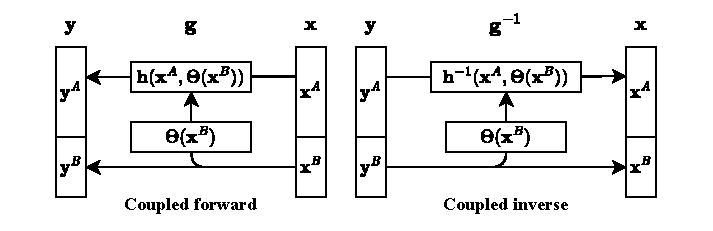
\includegraphics[width=0.95\textwidth]{figures/couplingflow.pdf}
  \end{center}
  \caption{Coupling flow operates on two partitions of the input
  $\mathbf{x} = [\mathbf{x}^A, \mathbf{x}^B]$, with $\mathbf{x}^B$ keep intact while $\mathbf{x}^B$ is \textit{coupled} with $\Theta(\mathbf{x}^B)$ by a \textit{coupling function} $\mathbf{h}$. Notice that the \textit{conditioner} $\Theta(\cdot)$ is not require to be inverted and thus can be arbitrary complex.}
  \label{fig:couplingflow}
\end{figure}


The expressive power of coupling flows resides in the choice of the conditioner
$\Theta(\mathbf{x}^B)$, which can be arbitrary complex. In practice,
$\Theta(\mathbf{x}^B)$ is realized by some neural network architecture depending
on the domain. For
instance, for graph generation tasks, $\Theta$ is chosen to be a graph neural
networks \citep{zangMoFlowInvertibleFlow2020} while for images generation, a
shallow ResNet can be used \citep{kingmaGlowGenerativeFlow2018}.

\subsubsection{Multi-scale flows}

Conditioner $\Theta$ can also be independent of $\textbf{x}^B$ and simplified to
be constant. This is the premise of \textit{multiscale flow} introduced by
RealNVP \citep{dinhDensityEstimationUsing2017}. The idea is to construct the generator
$\textbf{g}$ as a composition of coupling flows that transform an
increasingly large partition of the input while keeping other dimensions
unchanged. In the normalizing direction, the number of dimensions involved in
computing the inverted flow decreases exponentially in each
step, which greatly reduces computational costs of transforming the full
high dimensional data distribution during inference.
\citep{kruseHINTHierarchicalInvertible2021} further improved upon the idea of
multiscale flows by introducing recursive hierarchical coupling flows that
keep the expressive form $\Theta(\mathbf{x_B})$ while preserve necessary parallelizability for fast
sampling and inference. The multiscale composite nature of this
flow also allows the capturing of high-order structure that exhibits certain
types of natural data such as images.

\subsection{Autoregressive flows}

Autoregressive flows can be considered as a non-linear generalization of
triangular linear flows with high capacity to model complex correlations between dimensions. First introduced by
\citep{kingmaImprovedVariationalInference2016}, autoregressive flow has become a popular choice
due to its high expressivity and sampling quality but at the cost of computation
time due to the iterative computation of autoregressive architectures. Nonetheless,
it is an important basis for developing more expressive
flows models with theoretical guarantee for universality (i.e. the induced
transformation can represent arbitrary complex mapping between
the distributions under some reasonable assumptions). In fact the
proof referred in Section \ref{f:uni} stemmed from the choice of the
transformation being autoregressive.

\subsubsection{Formulation}
Autoregressive flows can be considered as the extreme case of coupling flows
where the dimensions are completely partitioned into individual terms $x_1,
x_2,\ldots, x_d \in \mathbb{R}$. Consider the \textit{coupling function} which is now a scalar
bijection $h(
\cdot\,; \theta
): \mathbb{R} \to \mathbb{R}$. Then the autoregressive generator
$\mathbf{g}: \mathbb{R}^D \to \mathbb{R}^D$ models each entry of
the output $\mathbf{y} = \mathbf{g}(\mathbf{x})$ as:
$$
y_t = h(x_t, \Theta_t(\mathbf{x}_{<t}))
.$$
where $\Theta_t$ are also called \textit{conditioners} which map
$\mathbb{R}^{t-1}$ to parameter space of $h$. Note that in some literature, $h$ is
referred to as the \textit{transformer}, which is unrelated to the
Transformer architecture that utilizes the attention mechanism.
\citep{vaswaniAttentionAllYou2017}.

The expressivity of autoregressive flow can again be attributed by the
unboundedness in architectural complexity of $\Theta_t$, which can be arbitrary
nonlinear functions. In practice, $\Theta_t$ are parameterized by a single model
and the evaluation of $\mathbf{g}$ can be efficiently computed in a single pass
through given appropriate masking of input dimensions. This is the main idea
behind Masked Autoregressive Flow (MAF) proposed by
\citep{papamakariosMaskedAutoregressiveFlow2017}, in an attempt to make
autoregressive flows parallelizable in modern computing hardware.
\begin{figure}
  \begin{center}
    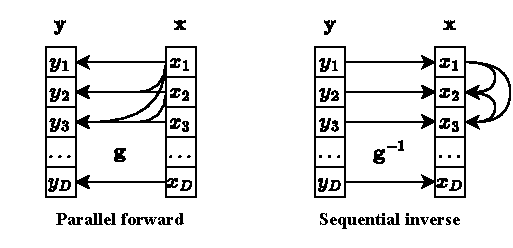
\includegraphics[width=0.7\textwidth]{figures/autoregressiveflow.pdf}
  \end{center}
  \caption{The computation of an autoregressive flow $\mathbf{g}(\mathbf{x})$
  can be parallelized by first
  produced $D$ masked inputs $x_1$, $[x_1, x_2]^T$, $\ldots$
  and compute $h(x_2, x_1)$, $h(x_3, [x_1, x_2]^T)$, $\ldots$ in parallel.
  The inverse $\mathbf{g}^{-1}(\mathbf{y})$ requires the inputs
  $\mathbf{x}_{<t}$ and thus must be sequential.}
  \label{fig:autoregressiveflow}
\end{figure}

The Jacobian of $\textbf{g}$ is a dense (lower) triangular matrix and hence
can be efficiently computed as the product of its diagonal entries:
$$
det \left(
\frac{\partial \mathbf{g}}{\partial \mathbf{x} }
\right) =  \prod_{t=1}^D \frac{dy_t}{dx_t}
.$$
However, while the generation direction can be computed in parallel as with MAF
,  the inverse can only be computed sequentially due to the dependence of
$x_{t}$ on $\textbf{x}_{<t}$:
$$
x_{t} = h^{-1}(y_t,
\Theta_t(\textbf{x}_{<t}))
.$$
which force the computation in the opposite direction
$\mathbf{g}^{-1}(\mathbf{y})$ to be sequential. Alternatively, the autoregressive dependence can be modified such that
$\Theta_t$ take $\mathbf{y}_{<t}$ as inputs which results in its inverse being a direct autoregressive flow:
\begin{align*}
  y_t &= h(x_t, \Theta_t(\mathbf{y}_{<t}))\\
  x_{t} &= h^{-1}(y_t, \Theta_t(\textbf{y}_{<t}))
\end{align*}

This formulation of autoregressive flows induce the opposite trade-off: relative
efficient computation of the inverse $\mathbf{g}^{-1}(\mathbf{y})$ at the
expense of non parallelizable evaluation of $\mathbf{g}(\mathbf{x})$. This is
the basis of Inverse Autoregressive Flows (IAF)
\citep{kingmaImprovedVariationalInference2016}. Thus, depending on the intended
applications, one might prefer the use of IAF or MAF for either faster sampling
or more efficient density estimation. Regardless of the decision, both methods
are based on the same principles and can be shown to be theoretical equivalents.

\subsubsection{Universality}

Autoregressive flows can be shown to be universal, i.e. capable of modeling
complex target distribution to arbitrary precision given sufficient data and
capacity \citep{jainiSumofSquaresPolynomialFlow2019,
huangNeuralAutoregressiveFlows2018} . As a corollary, an autoregressive flow
will possess such universality property if it can be demonstrated that its
coupling function $h$ is monotonic or the family of such coupling flows are
dense on the space of monotonic functions in pointwise convergence topology.

\subsection{Coupling functions}


The coupling function $\mathbf{h}(\cdot\,;\mathbf{\theta})$ is the primary
building block in constructing both coupling flows and autoregressive flows.
While they are defined as multivariate functions in coupling flows, they are
usually formulated as elementwise bijections for analytical tractability in
practice. Furthermore, in autoregressive flows, coupling functions are also
scalar functions and thus,  different choices of coupling functions on the
premise of them being simple scalar bijections $h: \mathbb{R} \to \mathbb{R}$
will be explored.

\subsubsection{Affine couplings}

NICE (nonlinear independent component estimation)
\citep{dinhNICENonlinearIndependent2015} contained some of the earliest proposals
of coupling functions, which are \textit{additive coupling function}:
$$
h(x\,;\theta) = x + \theta \quad \theta \in  \mathbb{R}
.$$
and \textit{affine coupling function}:
$$
h(x\,;\theta) = \theta_1 x + \theta_2 \quad \theta_1 \neq 0,
\theta_2 \in  \mathbb{R}
.$$

The efficient computation and simplicity leads affine couplings to be widely
used in flow literature. However, they have limited expressivity and thus
many consecutive flows need to be composed to represent complicated
distribution. When designing $\mathbf{h}(\cdot\,;\theta)$, as alluded in Section
\ref{f:uni}, one might ensure its monotonicity for theoretical guarantee of
universality. Therefore, it is frequent for \textit{affine coupling
flows} to be formulated such that $\theta_1 > 0$, which results in the following alternative forms for coupling and autoregressive flows respectively:
$$
\mathbf{h}(\mathbf{x}_B\,;\Theta, \mathbf{x}_A) = \mathbf{x}_B \odot e^{\mathbf{s}(\mathbf{x}_A\,;\Theta_1)} +
\mathbf{t}(\mathbf{x}_A\,;\Theta_2)
.$$
$$
h(x_t\,;\Theta, \mathbf{x}_{<t}) = x_t \cdot e^{s(\mathbf{x}_{<t}\,;\Theta_1)} +
t(\mathbf{x}_{<t}\,;\Theta_2)
.$$
where $\Theta = (\Theta_1, \Theta_2)$ is a partitioned parameter of the
coupling function and $\mathbf{s}, \mathbf{t}: \mathbb{R}^d \to \mathbb{R}^{D-d}$
(or $s, t: \mathbb{R}^d \to \mathbb{R}$ in elementwise form) are
arbitrary functions which are usually parameterized by neural networks with
weights $\Theta_1$ and $\Theta_2$.
Note that $\mathbf{s}$ and $\mathbf{t}$ are sometimes called the \textbf{scale
function} and \textbf{translation function}. The inverse of $\mathbf{h}$ in coupling flows is
efficient as $\mathbf{y}_A = \mathbf{x}_B$:
\begin{align*}
  \mathbf{h}^{-1}(\mathbf{y}_B\,;\Theta, \mathbf{x}_A)
  &= (\mathbf{y}_B - \mathbf{t}(\mathbf{x}_A\,;\Theta_2)) \odot
  e^{-\mathbf{s}(\mathbf{x}_A\,;\Theta_1)} \\
  &= (\mathbf{y}_B -
  \mathbf{t}(\mathbf{y}_A\,;\Theta_2)) \odot e^{-\mathbf{s}(\mathbf{y}_A\,;\Theta_1)}
\end{align*}
$$
  h^{-1}(y_t, \Theta, \mathbf{x}_{<t}) = (y_t - t(\mathbf{x}_{<t}\,;\Theta_2)) \cdot
  e^{-s(\mathbf{x}_{t}; \Theta_1)}
.$$

However, for autoregressive flows, the sequential dependence hinders much
parallel optimization. Representative works of affine coupling functions for
coupling flows includes the work of \citep{dinhNICENonlinearIndependent2015} on
NICE and \citep{dinhDensityEstimationUsing2017} on RealNVP, with expansion to
more the image generation domain with Glow \citep{kingmaGlowGenerativeFlow2018}.
Glow in particular, is a pivotal publication for normalizing flows as it
established flows as capable generative models with samples quality comparable
to GANs and VAEs at the time. For autoregressive flows, the publications of IAF
and MAF \citep{kingmaImprovedVariationalInference2016,
papamakariosMaskedAutoregressiveFlow2017} are notable examples of affine
coupling functions used in autoregressive transformations.

\subsubsection{Nonlinear couplings} There have been many research efforts in
constructing nonlinear complex couplings capable of more expressivity and
modeling power. For example, \citep{zieglerLatentNormalizingFlows2019} proposed
the ideas of nonlinear squared flow, where the invertibility of the
transformation is ensured as the resulting analytical computation contains
solving a cubic polynomial with unique real solution. Another example is Flow++,
where \citep{hoFlowImprovingFlowBased2019} further improved upon the idea of
affine couplings by introducing an additional invertible transformation based on
CDFs of $K$ logistics mixture: $$ h(x;\theta) = \theta_1 F(x, \theta_3) +
\theta_2 .$$ $$ F(x,\bm{\pi}, \bm{\mu}, \mathbf{s}) =
\sigma^{-1}\left(\sum_{j=1}^{K}\pi_j\sigma
\left(\frac{x-\mu_j}{s_j}\right)\right) .$$ The inverse of such flows does not
possess an analytical form but can be computed numerically via fixed-point
iteration (e.g. bisection algorithm). The upside to using monotonic mixture of
such CDFs is the derivatives are logistic PDFs with inexpensive evaluation.
Experimental ablation study showed that such modification improves performance
slightly.

Another approach to constructing monotonic nonlinear coupling functions is to
use \textit{splines} of various degrees. A spline is a piecewise polynomial
function defined by a set of points called \textit{knots} where the spline must
exactly cross. Denote this set of $K+1$ knots as $(x_i, y_i)_{i=0}^K$. For a
spline to be monotonic, which we will further assume to be increasing (without
the loss of generality), the set of knots must have $x_i < x_{i+1}$, $y_i <
y_{i+1}$ for $i=0,\ldots,K-1$. Interpolating between two or more consecutive
knots with monotonic polynomials of degree $P$ results in a valid monotonic
coupling function. For $P=1,2$ we have linear and quadratic monotone splines
\citep{mullerNeuralImportanceSampling2019}. For $P=3$ we have cubic monotone
splines, usually seeded with the derivatives at the two end points and
constructed via the Steffen's method \citep{durkanCubicSplineFlows2019}. Note
that splines are usually defined on compact intervals such as $[0,1]$ and thus
it is common that $h(x\,;\theta) = \sigma(\hat{h}(x\,;\theta)), \hat{h}: [0,1]
\to [0,1]$ where $\hat{h}$ is a surrogate spline to ensure the right range of
$h$.

Intuitively, it seems desirable to model $h$ as a neural network due to the
universal approximation theorem. \citep{huangNeuralAutoregressiveFlows2018}
follows this approach to devise Neural Autoregressive Flow (NAF) where $h(\cdot;
\theta)$ is parameterized by a multi layer perceptron (MLP). Indeed, the
resulting autoregressive flows possess universality property. In general, as
formally shown by the authors, MLP are not invertible but under sufficient
conditions on its weights, the learned MLP can be monotonic and thus reversible.
unconstrained MLP and thus require more complex conditioner for the same
modeling performance. \citep{wehenkelUnconstrainedMonotonicNeural2019} proposed a
solution to such problem by relax the requirements to strictly-positive-output
MLPs and integrate numerically to produce monotonic increasing functions.

\citep{jainiSumofSquaresPolynomialFlow2019} suspected
$h$ is overparameterized if modeled as MLPs and thus proposed a
simpler coupling function computed by summing squared polynomials and then integrate:
$$
h(x\,;\theta) =  \int_{0}^x \sum_{k=1}^K \left(\sum_{l=0}^L a_{kl}u^l \right)^2 du
.$$

The resulting sum-of-square polynomial flows are named SOS
\citep{jainiSumofSquaresPolynomialFlow2019} and experimentally are easier to
train compared to NAF due to the unconstrained nature of parameters $a_{kl}$.
Note that $K$ and $L$ are hyperparameters that can be chosen beforehand to tune
expressivity at the risk of over/under-fitting. When $L=0$, SOS reduces to
\textit{affine coupling functions} and can be considered as a generalization of
affine coupling flow. It was also formally proven by
\citep{jainiSumofSquaresPolynomialFlow2019} that such flow is indeed universal
and can transform the base distribution to arbitrarily complex distribution.

\section{Continuous flows}
\subsection{Background}
Continuous flows can be considered as a continuous-time generalization of
residual flows, which in turn, inspired by the idea of residual
networks \citep{heDeepResidualLearning2016}. Such networks are composed of functions of the form:
\begin{align}
\label{f:res}
\mathbf{g}(\mathbf{x}) = \mathbf{x} + F(\mathbf{x})
\end{align}

Here $\mathbf{g}(\mathbf{x})$ are called a \textit{residual connection} and
$F(\mathbf{x})$ is usually a neural network. Specifically, the original
ResNet \citep{heDeepResidualLearning2016} parameterized $F(\mathbf{x})$
as blocks of CNNs followed by a batch normalization layer. Flow networks that
utilize composition of such residual connections are usually referred to as
\textit{residual flows}.

Residual flow is essentially a discrete version of the more general so-called
\textit{continuous} or \textit{infinitesimal} flows \citep{chenNeuralOrdinaryDifferential2019}, which model the process of
transformation as a continuous time dependent function rather than a discrete
composition of residual connections $\mathbf{g}$. Such function is the solution to the
initial-value problem of an ordinary differential equation (ODE):
\begin{align}
\label{f:ode}
  \frac{d \mathbf{x}(t)}{d t} =
  F(\mathbf{x}(t), \theta(t))
\end{align}
Propagating through such networks requires
solving an ODE via a black-box solver to find the evaluation of the function at
a predefined endpoint in time. This approach to model continuous
infinite flows (or infinite depth neural networks) has spawned a novel branch of
research in normalizing flows with potential higher modeling capacity and lower
memory requirements to store intermediate parameters.
\subsection{Formulation}

Consider the initial value problem for the ODE given in Equation \ref{f:ode}. In
the generative direction, let $t \in [0,1]$ and initial condition $\mathbf{x}(0)
= \mathbf{z}$. Assuming Lipschitz continuity of $F$ in $\mathbf{x}$ and
continuity in $t$, then the solution exists and is unique
\citep{arnoldOrdinaryDifferentialEquations1992}, which in turn, reaffirms that
the solution set consists of invertible functions. Now denote the solution at
each time $t$ as $\Phi^t(\mathbf{z})$. Define the solution at $t=1$ as the
generator (i.e. $\Phi^1(\mathbf{z}) = \mathbf{g}(\mathbf{z}) = \mathbf{y}$).
Intuitively, this gives a way to model $\mathbf{g}(\mathbf{z})$ as a dynamic
process through time $t$ with output as the process's state at $t=1$. Modeling
the generator as $\Phi^1(\mathbf{z})$ (also called the \textit{time-one map})
and solving it via black-box solvers was the idea behind NODE (Neural ODE)
\citep{chenNeuralOrdinaryDifferential2019}.

\textit{Remarks: } In mathematical formalism, the solutions $\Phi^t(\cdot):
\mathbb{R}^D \to \mathbb{R}^D$ form a one-parameter \textit{group} of diffeomorphism
$(\mathcal{P}, \circ)$, where $\circ$ is the composition operator (i.e. $\Phi^t
\circ \Phi^s = \Phi^{t+s} \in \mathcal{P}, t+s \leq 1$). Furthermore, from the
perspective of neural networks, this can be considered as an "infinite depth"
(residual) neural network with input $\mathbf{z}$ and output $\mathbf{y}$,
parameterized by continuous time-dependent weights $\theta(t)$.

The primary concern regarding this method of continuous transformation is how
to propagate the gradients needed for optimization on supervised tasks. Since
gradients can not be trivially propagated through the computation of ODE
solvers, the \textit{adjoint sensitivity method} is used as a tractable
replacement. Logically, the method can be considered as a continuous analogy of
the backpropagation: if the gradient at the $n$-th hidden layer in a neural
network is $\frac{dL}{d \textbf{h}_n} = \frac{dL}{d \mathbf{h}_{n+1}} \frac{d
\mathbf{h}_{n+1}}{d \mathbf{h}_n}$ then the algebraic-continuation
time-dependent gradient $\mathbf{a}(t)$ must satisfy the augmented ODE:

$$
\frac{d\mathbf{a}(t)}{dt} = -\mathbf{a}(t) \frac{dF(\mathbf{x}(t),
\theta(t))}{\mathbf{x}(t)}
.$$
where $\mathbf{a}(t) = \frac{dL}{d\mathbf{x}(t)}$ is also called the \textit{adjoint} or
\textit{sensitivity}.

For density estimation however, we do not have a loss but instead aim to
maximize the log likelihood. The continuous log-likelihood
at each time step $t$ is now also given as solution to another ODE analogous to
the change of variable formula:
$$
\frac{d}{dt}\log(p(\mathbf{x}(t))) =
-\text{Tr}\left(\frac{dF(\mathbf{x}(t))}{\mathbf{x}(t)}\right)
.$$
The log likelihood of a data point $\mathbf{y}$ is computed by first solve the
reverse ODE to yield the corresponding $\mathbf{z}$ and then solve the "change of
variable" ODE above at $t=1$ (i.e. $p_{\mathbf{Y}}(\mathbf{y}) =
p(\mathbf{x}(1))$), given the initial-value $p(\mathbf{x}(0)) =
p_{\mathbf{Z}}(\mathbf{z})$.
Note that the determinant is no longer needed in the formula and thus is
theoretically less expensive to compute.

\citep{grathwohlFFJORDFreeformContinuous2018} further compliment NODE with the
following works of FFJORD, which improved upon the existing continuous change of
variable formula by introducing Hutchinson estimator to approximate the trace
term for faster evaluation. \citep{finlayHowTrainYour2020} introduced two
regularization terms to the loss function of FFJORD, which was the Frobenius
norm of the Jacobian $det\left(\frac{dF(\mathbf{x}(t))}{\mathbf{x}(t)}\right)$
and a forcing term that limits the solution trajectories to follow straight
paths with zero acceleration. A promising finding of using continuous flows in
comparison to discrete composite flows is the efficient use of parameters. A
comparison experiment suggested that on the CIFAR10 dataset, for comparable
performance, FFJORD requires less than $2\%$ as many parameters as Glow.


However, there are certain limitations with continuous flows that have been
recognized, specifically focused on the corresponding Jacobian of such flows.
Since the defined ODE traces a continuous path in the space of diffeomorphism
(which consists of functions with nonzero Jacobian determinant) that starts from the identity solution at
time-zero i.e. $\Phi^0(\mathbf{z}) = I\mathbf{z}$ to the time-one map
i.e. $\Phi^1(\mathbf{z}) = \mathbf{y}$, it is necessary that
$det\left(\frac{d\Phi^t(\mathbf{z})}{d\mathbf{z}}\right) \forall t \in [0,1]$
share the same sign. Since
$det\left(\frac{d\Phi^0(\mathbf{z})}{d\mathbf{z}}\right) = det(I) > 0$, it is
necessary that at all time step $t$, the Jacobian of the solution
$\Phi^t(\mathbf{z})$ is positive or in order words, \textit{orientation preserving}. This
is an inescapable subspace of the space of all possible transformations with positive and
negative Jacobian and thus can be considered a limitation in expressivity of
NODEs. A novel solution to this problem is to consider an \textit{augmented} version of
NODE (ANODE) that can represent a more inclusive class of diffeomorphisms by adding
"slack" variables $\tilde{\mathbf{x}}(t) \in \mathbb{R}^p$ and consider the
\textit{augmented} ODE \citep{dupontAugmentedNeuralODEs2019}:
$$
\frac{d}{dt} \begin{bmatrix}
  \mathbf{x}(t) \\
  \tilde{\mathbf{x}}(t)
\end{bmatrix} = \tilde{F}\left( \begin{bmatrix}
  \mathbf{x}(t) \\
  \tilde{\mathbf{x}}(t)
\end{bmatrix}, \theta(t)\right)
.$$
\citep{dupontAugmentedNeuralODEs2019} suspected that such addition of a slack
variable allows for the Jacobian of the solutions to wander more freely to the
negative domain, permitting the learning of distributions that previous NODE incapable of
representing. This hypothesis seemed to be reflected in the papers' quantitative
experiments with an additional surprise of shorter training time. In fact, it
has been formally proven by \citep{zhangApproximationCapabilitiesNeural2020} that
the space of all possible transformations is covered by ANODE and thus the
resulting continuous flows are indeed universal.


\chapter{Graph Neural Network}
\label{c:gnn}

\section{Background}
Graph neural networks (GNNs) in their most general definition can be considered
as composite DL-inspired methods that account for permutation
invariant property and thus are operable on graphs. There have been multiple surveys
published in effort of standardizing and categorizing GNNs
\citep{zhangdeeplearninggraphs2020, zhouGraphNeuralNetworks2020,
chamiMachineLearningGraphs2022, gilmerNeuralMessagePassing2017}. In
an effort of contributing a bird-eye overview of GNNs , this thesis begins the
journey of categorizing different architectures by looking through the
high-level lens of deep learning architectural design. Similar to common CNNs
architectures, GNNs can be considered as computing pipelines, composed of
\textit{computational modules} that fall into three main categories:
\textit{propagation modules}, \textit{sampling modules} and \textit{pooling
modules} \citep{zhouGraphNeuralNetworks2020}. Propagation modules can be
considered as the central information aggregators that through the process of
propagating information between nodes, are capable of capturing latent feature
and topological information underlying each graph. Sampling modules, on the
other hand, are stochastic sampling regimes that are designed more specifically
to graph to solve the exponential expansion of the receptive field of each node
during propagation. Finally, pooling modules are essential analogs of pooling
layers in CNNs that reduce dimensionality and extract high level features of
otherwise multidimensional intermediate representations of graphs. The
downstream output after subsequent combinations of these computational modules
are usually latent representation of graphs (i.e. embeddings) that can be used
for classification, clustering, outlier detection and most relevantly,
generative modeling. Here, an emphasis is placed on graph propagation
modules, as they are the primary actors operating on relational data in
molecule generation with normalizing flows.

To explore various propagation modules, this thesis employs the unification
framework of \textit{Message Passing Neural Network} (MPNNs), which grouped
various GNNs architecture that share the same information propagation strategy
of sending messages between neighboring vertices. This can be seen as an
instance of \textit{spatial methods} that utilize the spatial information imbued
by the 2D planar representation of graphs. Conversely, \textit{spectral
approaches} leverage graph Fourier transform to shift the perspective from
propagating information in the spatial graph domain to convolution operation in
the spectral domain. Spectral methods benefit from theoretical guarantees of
previous works in \textit{graph signal processing} and remain prominent among
researchers. Signature works that fall under this line of methods are Spectral
network \citep{brunaSpectralNetworksLocally2014}, Chebnet
\citep{defferrardConvolutionalNeuralNetworks2016}, GCN
\citep{kipfSemiSupervisedClassificationGraph2017}, AGCN
\citep{liAdaptiveGraphConvolutional2018} and DGCN
\citep{zhuangDualGraphConvolutional2018}. Curious readers can explore various
intricacies of spectral methods for graph representation learning in
\citep{zhouGraphNeuralNetworks2020}.

Propagation modules can also be explored from two orthogonal perspectives:
horizontally, i.e. how latent information is extracted in each processing layer
and vertically, i.e. how graph features permeate from one propagating layer to
the next. There are two main operators used in vertical (or depthwise)
propagation: convolution operators and recurrent operators
\citep{wuComprehensiveSurveyGraph2021}. The main distinction between the two
approaches is the reusing of parameters during propagation between layers. While
convolution uses separate weights for each operating layer, recurrent approaches
recycle the weights and autoregressively pass the previous output as the next
input. Consequently, the notion of layer depth and time are mostly applied to
convolution methods and autoregressive methods respectively and are rarely
interchangeable, which is later exemplified by formulation of MPNNs and their
derivatives. Notable works in modeling layers of graphs transformation as
sequential recurrent processes mostly consist of applying gated mechanisms (e.g.
GRUs and LSTMs) to graphs using various type of GNNs as computation modules
(e.g. GGNN \citep{liGatedGraphSequence2017} and Graph LSTM
\citep{zayatsConversationModelingReddit2018}).

In an effort to scope the evolving field of GNN that is relevant to molecule
generation, only common approaches to GNN in molecule generation are explored in
detail in this section. The exploration follows the path of categorization of
MPNN, as laid out by \citep{gilmerNeuralMessagePassing2017}. Also, note that
there is an implicit assumption of undirected non dynamic graphs to simplify the
formulation of MPNNs and their examples. In other words, directed graphs and
dynamic graphs that evolve over time are not covered in this section but should
be extrapolated reasonably well to other types of graph under slightly modified
constructions.

\section{The Message Passing Framework}
\subsection{Formulation}

Denote a graph as $\mathcal{G} = (\mathcal{V}, \mathcal{E}, \mathbf{V}, \mathbf{E})$,
where $\mathcal{V}$ is the set of vertices, $\mathcal{E}$ is the set of edges,
$\mathbf{V} \in \mathbb{R}^{N \times d_1}$ is the node feature matrix and
$\mathbf{E} \in \mathbb{R}^{N \times N \times d_)}$ is the edge feature matrix.
At input, each vertex $v$ is accompanied by a node feature vector
$\mathbf{x}_v^0 \in \mathbb{R}^{d_1}$ and each edge between two vertices $v,w$
is accompanied by an edge feature vector $\mathbf{e}_{vw} \in \mathbb{R}^d_2$.
For simple graphs with no edge attributes, $\mathbf{E} \in \mathbb{R}^{N \times
N}$ is the adjacency matrix (i.e. $\mathbf{E}_{[i,j]} = e_{vw}= 1$ if there exists
an edge between the $i$-th vertex $v$ and $j$-th vertex $w$ and $0$ otherwise).
MPNN describes the graph propagation step as a time parameterized two phase
process: the \textit{message passing phase} and the \textit{update phase},
indicated by the following two equations:
\begin{align}
  \mathbf{m}_{v}^{t+1} &= \underset{w \in N(v)}{\text{Agg}} M_t(\mathbf{x}_v^t,
\mathbf{x}_w^t, \mathbf{e}_{vw}) \\
  \mathbf{x}_v^{t+1} &= U_t(\mathbf{x}_v^t, \mathbf{m}_{v}^{t+1})
\end{align}
Here $M_t$ are the message passing functions, $U_t$ are the vertex update
functions and $\text{Agg}$ is an \textit{aggregating function} that is
permutation invariant with respect to its parameters. Common choices of
$\text{Agg}$ are argmax, sum and product. After the message was "passed" or
computed from neighboring vertices' features $\mathbf{x}_{w}^t$ and the relevant
connecting edge features $\mathbf{e}_{vw}$, the next phase is to compute the new
hidden feature with $U_t$ given the message and the previous hidden
feature $\mathbf{x}_{v}^{t}$ as parameters.

\begin{figure}
  \begin{center}
    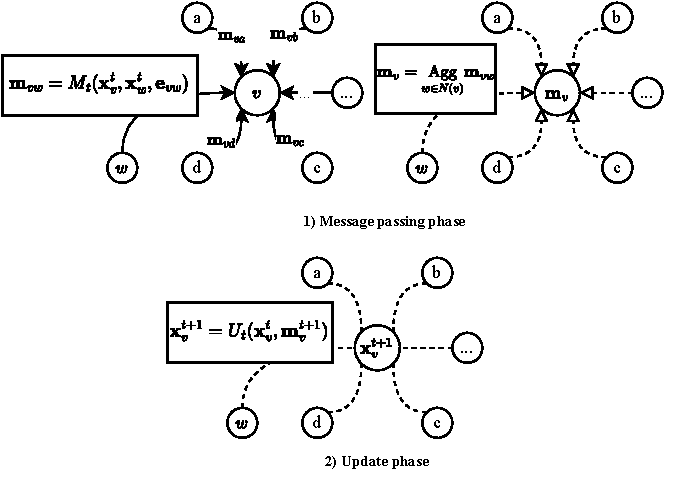
\includegraphics[width=0.95\textwidth]{figures/mpnn.pdf}
  \end{center}
  \caption{The computation of an MPNN layer consists of two phase: the
  \textit{message passing phase} and the \textit{update phase}. The
  message passing phase update aggregate the \textit{messages}
  $\mathbf{m}_{vw}$ from the neighboring vertices $w$ of $v$ aggregate them
  with an aggregation function $\text{Agg}$.}
  \label{fig:}
\end{figure}


The processing step is repeated from $t=0$ until $t=T$, with larger $T$ indicates the
information of vertices gets more and more dispersed in the graph. Concretely,
the \textit{receptive fields} of each vertex, i.e., the set of vertices whose
features were used in the computation of its message (at the current and
previous message passing phase) get exponentially larger for bigger $T$. The
fact that receptive fields radius grows exponentially with $T$ poses a problem
for GNNs to learn localized

The original paper also proposed an optional \textit{readout phase} after $T$ steps
of message passing propagation, which computes a global feature that encompassed all hidden
features of the graph's vertices:
$$
  \mathbf{x}_{\mathcal{G}} = R(\{\mathbf{x}_{v}^T |\, v \in \mathcal{G}\})
.$$
where $R$, usually referred to as the \textit{readout function}, must also be
permutation invariant as required for MPNN to be invariant to graph isomorphism.
Furthermore, for optimization, it is also required that $U_t$, $M_t$ and $R$ are
learnable differentiable functions. Note that the original works only
formulate $\mathbf{e}_{vw}$ as a binary value (i.e. an adjacency matrix entry)
corresponding to an unattributed edge with no edge features. This is due to the
contemporary research landscape at the time not involving much exploration of MPNNs
utilizing edge features as well as large molecular datasets that store edge
features.

The original paper of MPNNs also includes various experimental variants of
MPNNs that promote distant information propagation and decreasing computational
cost. Notable ideas include adding virtual edges between distant vertices
; using latent master node fully connected to every other vertices to serve as a
temporary memory space; and multiple towers architecture that splits vertex embeddings
$\mathbf{x}_{v}^t \in \mathbb{R}^{d_1}$ into $k$ distinct vectors
$\mathbf{x}_{v}^{t,k} \in \mathbb{R}^{d_1/k}$, then runs the propagation step on each of
the $k$ copies separately to get temporary features
$\{\hat{\mathbf{x}}_v^{t+1,k}, v \in \mathcal{G}\}$ (with separate message and
update functions $M_t^k, U_t^k$) and finally merge all temporary embeddings
together with a neural network $f$:
$$
  \mathbf{x}_{v}^t = f(\hat{\mathbf{x}}_v^{t,1}, \ldots, \hat{\mathbf{x}}_v^{t,k})
.$$

Disregarding the edge features, the multiple tower setup reduces the worst-case
computation complexity on dense graphs from $O(n^2d_1^2)$ to $O(n^2d_1^2/k)$, which is useful
for larger molecules since it allows for larger hidden states for the same number
of parameters.

\subsection{Examples}

\subsubsection{Neural FPs \citep{duvenaudConvolutionalNetworksGraphs2015}} The
original work of Neural FPs was motivated from the needs for a differentiable
computation of \textit{graph fingerprints}, specifically, the existing
extended-connectivity circular fingerprints (ECFP) \citep{rogersExtendedConnectivityFingerprints2010} was a discrete
refinement of the Morgan algorithm \citep{morganGenerationUniqueMachine2002} and thus unsuitable for gradient
optimization. The message passing used in the paper is a simple concatenation
$M(\mathbf{x}_v, \mathbf{x}_w, \mathbf{e}_{vw}) = [\mathbf{x}_w ||
\mathbf{e}_{vw}]$ and the update function is a linear transform composed with
the sigmoid function $U_t(\mathbf{x}_v^t, \mathbf{m}_v^{t+1}) =
\sigma(\mathbf{H}_t^{|N(v)|}\mathbf{m}_{v}^{t+1})$. The aggregating function is
the simple sum over neighboring vertices $\text{Agg} = \sum_{w \in N(v)}$. The
learnable matrix $\mathbf{H}_{t}^{|N(v)|}$ is degree specific (i.e., vertices
with the same degree share the same $\mathbf{H}_t^{|N(v)|}$), which serves as a
balance decision of model parameterization. However, the choice of concatenation
for the message function $M_t$ results in problematic separation of node and
edge features $\mathbf{m}_v^{t+1} = [\sum \mathbf{x}_w^t || \sum \mathbf{e}_{vw}]$.
Therefore, it follows that the Neural FPs implementation by
\citep{duvenaudConvolutionalNetworksGraphs2015} is incapable of capturing
correlations between nodes and edges signatures.

\subsubsection{GG-NN \citep{liGatedGraphSequence2017}} The message passing
function is a simple edge-specific linear transformation of neighboring node
features $M_t(\mathbf{x}_v^t, \mathbf{x}_wa^t, \mathbf{e}_{vw}) =
\mathbf{H}_{\mathbf{e}_{vw}} \mathbf{x}_w^t$ where $A_{\mathbf{e}_{vw}}$ are
learnable matrices. Here the edges are assumed to be categorical (i.e. there is
only a specific set of possible edge types). The update function is modeled as a
Gated Recurrent Unit (GRU) \citep{chungEmpiricalEvaluationGated2014}
$U_t(\mathbf{x}_{v}^t, \mathbf{m}_{v}^{t+1}) = \text{GRU}(\mathbf{x}_{v}^t,
\mathbf{m}_{v}^{t+1})$ and can be seen as an instance of recurrent operators
rather than convolution operators for vertical graph propagation.

\subsubsection{GraphSAGE \citep{hamiltonInductiveRepresentationLearning2017}}
GraphSAGE can be seen as a general inductive framework that generates embeddings
with message passing but with the additional steps of localized neighborhood
sampling. The aggregating function $\text{Agg}$ is relaxed to account for a
larger family of aggregators including autoregressive aggregators such as LSTMs
and GRUs as well as mean and pooling aggregators. Moreover, rather than
aggregate over all neighboring vertices, a fixed-size sample of the vertex's
neighborhood is used for aggregating information instead. This mitigates the
exponential widening of the receptive fields and therefore reduces oversmoothing
in practice. The messaging phase is thus represented by the following equation
instead: $$ \mathbf{m}_{v}^{t+1} = \underset{w \in
\mathcal{S}(N(v))}{\text{Agg}^{t+1}} \mathbf{x}_{w}^t = \text{Agg}^{t+1}(\{
  \mathbf{x}_w^t, w \in \mathcal{S}(N(v))\}) .$$ where $\mathcal{S}$ denotes the
sampler function that produces a uniformly sampled subset of $N(v)$. It can be
shown that GraphSAGE with a mean aggregator performed the same as an inductive
version of Graph Convolution Network (GCN)
\citep{kipfSemiSupervisedClassificationGraph2017}. Furthermore, the use of LSTMs
as aggregators does not guarantee the permutation invariant requirements needed
in GNNs and thus requires specific reordering of the vertices. Notably, the
updating function is similar to Neural FPs, except the matrix $\mathbf{W}$ used
in linear transformation being reused in each processing step:
$$
\mathbf{x}_{v}^{t+1}= U_t(\mathbf{x}_{v}^{t}, \mathbf{m}_{v}^{t+1}) = \sigma(\mathbf{W}^{t+1}[\mathbf{x}_{v}^t || \mathbf{m}_{v}^t])
$$
where $[\,\cdot\, ||\, \cdot\,]$ indicates concatenation. Intuitively, this
formulation of $U_t$ decrease the parameter count of the final model and better
training efficiency.



\subsubsection{GCN \citep{kipfSemiSupervisedClassificationGraph2017}} Motivated
from the convolution operator from the image domain, GCN aims to perform
convolution in the spectral representation of graph and is a prominent instance
of successful application of spectral methods. Consider the graph normalized
Laplacian $\mathbf{L} = \mathbf{I}-\mathbf{D}^{-1/2}\mathbf{A}\mathbf{D}^{-1/2}$
where $\mathbf{A} = \mathbf{E}_{::1}$ is the adjacency matrix, $\mathbf{D}$ is
the degree matrix (i.e., $\mathbf{D}_{ii} = |N(v_i)|,\, \mathbf{D}_{[i,j]} =
0,\, \forall i \neq j$). Since the graph Laplacian $\mathbf{L}$ is symmetric
positive semidefinite, one can perform the eigendecomposition $\mathbf{L} =
\mathbf{U\Lambda U^T}$ where $\mathbf{U}$ is an orthogonal matrix with
$\mathbf{L}$'s eigenvectors as columns and$\mathbf{\Lambda}$ is a diagonal
matrix of $\mathbf{L}$'s eigenvalues. Here one can define the graph Fourier
transform of a signal $\mathbf{x}$ on the corresponding graph $\mathcal{G}$ as
follows: $$ \mathfrak{F}(\mathbf{x}) = \mathbf{U}^T \mathbf{x} \quad , \quad
\mathfrak{F}^{-1}(\mathbf{x}) = \mathbf{U} \mathbf{x} .$$ The resulting
convolution operation on the spectral domain after the graph Fourier
transformation, according to the convolution theorem
\citep{mallatWaveletTourSignal1999}, can be defined as: \begin{align}
  \label{eq:fourier} \mathbf{f} * \mathbf{x} =
  \mathfrak{F}^{-1}(\mathfrak{F}(\mathbf{f}) \odot \mathfrak{F}(\mathbf{x}) =
  \mathbf{U}(\mathbf{U}^T \mathbf{f} \odot \mathbf{U}^T \mathbf{x}) \end{align}
  where $\mathbf{U}^T \mathbf{f}$ is also referred to as the \textit{spectral
  filter}. Given $f$ as a learnable transformation, preferably a parameterized
  function corresponding to a simple elementwise transformation (denoted as
  $\mathbf{f}_{\theta}$), the convolution operation in (\ref{eq:fourier}) can be
  simplified to: $$ \mathbf{f}_{\theta} * \mathbf{x} = \mathbf{Uf}_{\theta}
  \mathbf{U}^T \mathbf{x} .$$

Previous spectral works predates GCN proposed various approximation schemes of
$\mathbf{f}* \mathbf{x}$, for instance, direct parameterization as a diagonal
matrix $\mathbf{f} * \mathbf{x} = \text{diag}(\mathbf{w}) * \mathbf{x}$
\citep{brunaSpectralNetworksLocally2014} and using of Chebyshev polynomials up to the $K$-th
order \citep{defferrardConvolutionalNeuralNetworks2016}. GCN introduce the approximation $\mathbf{f}_{\theta} *
\mathbf{x} = \mathbf{Uf}_{\theta} \mathbf{U}^T \mathbf{x} \approx w
\mathbf{U\Lambda}\mathbf{U}^T \mathbf{x} = w \mathbf{L}\mathbf{x}$ and the
\textit{renormalization trick} $\mathbf{L} =
\mathbf{I}-\mathbf{D}^{-1/2}\mathbf{A}\mathbf{D}^{-1/2} \to
\tilde{\mathbf{D}}^{-1/2} \tilde{\mathbf{A}}\tilde{\mathbf{D}}^{-1/2}$ where
$\tilde{\mathbf{A}} = \mathbf{A} + \mathbf{I}$ and $\tilde{\mathbf{D}}_{ii} =
\sum_{j}\tilde{\mathbf{A}}_{[i,j]}$, which helps with the exploding/vanishing
gradient problem in practice. Here $w \in \mathbb{R}$ is a learnable parameter.
Under the MPNN framework, GCN's propagation step can be modeled as:
\begin{align*}
  M_t(\mathbf{x}_v^t, \mathbf{x}_w^t) &=
  (|N(v)||N(w)|)^{-1/2}e_{vw}\mathbf{x}_{w}^t \\
  U_t(\mathbf{x}_{v}^t, \mathbf{m}_{v}^{t+1}) &= \text{ReLU}(\mathbf{W}^t
  \mathbf{m}_{v}^{t+1})
\end{align*}
Here assuming there are no edge features and $e_{vw}$ is the corresponding
entries in the adjacency matrix $\mathbf{A}_{[i,j]}$ and thus is binary.

\subsubsection{R-GCN \citep{schlichtkrullModelingRelationalData2018}}

Relational Graph Convolution Network (R-GCN)
\citep{schlichtkrullModelingRelationalData2018} was motivated from previous works
of GCNs and MPNNs, but motivated to extend to consider different edge types
(also referred to as \textit{relations types}) rather than the simple adjacency
information between edges (i.e. connected or disconnected) like GCNs. R-GCN
assumes the existence of a finite categorical set $\mathcal{R}$ of relations
types between any two vertices and defines each edge as a $3$-tuple of $(v, r,
w) \in \mathcal{E}$, where $r \in \mathcal{R}$ is some relation type. The
messaged information aggregated in each vertex is a normalized weighted sum over
neighboring vertices' features (after some relation-specific linear
transformation) and different relation types:
$$
\mathbf{m}_{v}^{t+1} = \sum_{r \in \mathcal{R}} \sum_{w \in N_r(v)}
\frac{1}{c_{v,r}} \mathbf{W}_{r}^t \,\mathbf{x}_{v}^t
.$$
where $N_r(v)$ denotes the set of neighboring vertices under the relation $r \in
\mathcal{R}$ and $c_{v,r}$ is the normalization constant that can be learned or
chosen in advance (e.g. $c_{v,r} = |N_r(v)|$). The updating phase consists of a
basic addition and non-linear transformation, which is usually a
$\text{ReLU}(\cdot) = \text{max}(0, \cdot)$:
$$
\mathbf{x}_{v}^{t+1} = \text{ReLU}(m_{v}^{t+1} + \mathbf{W}^t \mathbf{x}_{v}^t)
.$$
where $\mathbf{W}^t$ is a common weight matrix shared between all message
passing computation of the graph's vertices.

\textit{Remarks}: R-GCNs is a popular choice of architecture among deep
molecular generation research due to their simplicity and being easily scalable to
large datasets. Despite being simple, stacking multiple layers of R-GCNs can
achieve high expressivity without the risk of oversmoothing. Intuitively, this
can be attributed to the fact that different relations possess separate sets of
learnable weights and in combination, can be considered as an ensemble of different GCNs.

\subsubsection{GAT \citep{velickovicGraphAttentionNetworks2018}}

The attention mechanism is a popular feature-mixing paradigm inspired from human
cognitive ability to focus and shift attention from/to various subjects
conditionally. Its popularity as an architectural abstraction stemmed from being
the primary mechanism behind the novel \textit{Transformer} architecture
\citep{vaswaniAttentionAllYou2017}, which has shown impressive capacity to model
complex unstructured relation in natural language, specifically long distance
relationships that are non trivial to efficiently model using existing
sequential approaches such as RNNs and LSTMs. Graph Attention Network (GAT)
\citep{velickovicGraphAttentionNetworks2018} constructed a weighing schemes
following the \textit{self-attention} strategy. Specifically, incoming messages
from neighboring vertices were weighted depending on their relevance to the
central vertex, conditioned on its current features $\mathbf{x}_{v}^t,
\mathbf{x}_w^t$. From the perspective of MPNN, in addition to the message
passing phase and updating phase, an was post hoc \textit{attending phase} was
required to compute the necessary attention weights, resulting in the total
propagation step consisting of three computing phases:
\begin{gather*}
  \alpha_{vw} = A_t(\mathbf{x}_{v}^t, \mathbf{x}_{w}^t)
  \\
  \mathbf{m}_v^{t+1} = \text{Agg}(\{\alpha_{vw}M_t(\mathbf{x}_{v}^t,
  \mathbf{x}_w^t) | \, w \in N(v)\}
  \\
  \mathbf{x}_v^{t+1} = U_t(\mathbf{x}_v^t, \mathbf{m}_v^{t+1})
\end{gather*}
For GAT, we have:
\begin{gather*}
  A_t(\mathbf{x}_{v}^t, \mathbf{x}_{w}^t) = \frac{
  \text{exp}(\text{LeakyReLU}(\mathbf{a}^T[\mathbf{W}\mathbf{x}_{v}^t ||
  \mathbf{W}\mathbf{x}_{w}^t]))
  }{ \sum_{k \in N(v)} \text{exp}(\text{LeakyReLU}(\mathbf{a}^T
    [\mathbf{W}\mathbf{x}_{v}^t]) || \mathbf{W} \mathbf{x}_{k}^t)
  } \\
  M_t(\mathbf{x}_v^t, \mathbf{x}_w^t) = \mathbf{W} \mathbf{x}_w^t \\
  U_t(\mathbf{x}_v^t, \mathbf{m}_v^{t+1}) = \rho(\mathbf{m}_v^{t+1})
\end{gather*}

\begin{figure}
  \begin{center}
    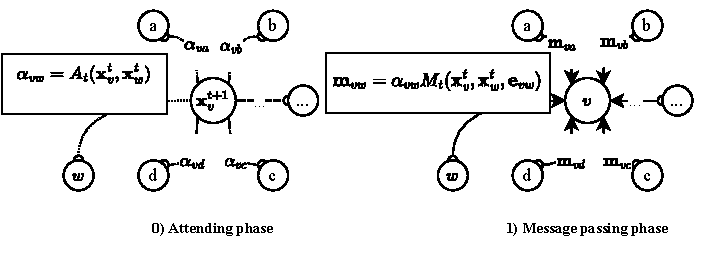
\includegraphics[width=0.95\textwidth]{figures/gat.pdf}
  \end{center}
  \caption{GAT infuse the attention mechanics with message passing, allowing
  central nodes to attend to important messages from neighboring nodes. With
  $H$ different matrices corresponding to $H$ different attending heads,
  multiple attention weights $(\alpha_{vw})_{i=1}^H$ are computed in parallel
  (\textit{multi-head attention}).}
  \label{fig:gat}
\end{figure}


where $\mathbf{W}$ is a learnable weight matrix associated with the linear
transformation performed on each vertex while $\mathbf{a}$ is the parameterized
vector of a single-layer multilayer perceptron (MLP). Note that $\text{Agg} =
\sum$, i.e. the common summing aggregator is used. In addition to the
self-attention mechanism, GATs also employ the use of \textit{multi-head
attention} proposed by \citep{vaswaniAttentionAllYou2017} to maximize modeling
capacity . Specifically, $K$ independent attention head matrices
$(\mathbf{W}_k)_{k=1}^K$ are used, each corresponding to a separate propagation
steps with independent attention weights, messages and updating functions. This
independence between each attention head also permits parallel computing schemes
that drastically improve training time despite the additional expressivity. With
different attention heads producing different intermediate feature state, a
mixing function is used to combine them and yield the final output feature for
one propagation step. With GAT, \citep{velickovicGraphAttentionNetworks2018}
proposed two methods for mixing attention heads: concatenation and mean
averaging:

$$
\mathbf{x}_{v}^{t+1} = \bigg\lvert\bigg\lvert_{k=1}^K \sigma\left(\sum_{w \in
N(v)}\alpha_{vw}^k \mathbf{W}_{k} \mathbf{x}_{u}^t\right)
.$$
$$
\mathbf{x}_{v}^{t+1} = \sigma\left(\frac{1}{K}\sum_{k=1}^K\sum_{w \in
N(v)}\alpha_{vw}^k \mathbf{W}_{k} \mathbf{x}_{u}^t \right)
.$$

This formulation of multi-head attention serves several advantageous properties:
computationally efficient due to ease in parallelizability of attention heads,
applicable to vertices of various degrees by assigning random weights to
neighboring vertices, and easily modifiable for inductive learning problems.

Future works on attention-based spatial GNNs mostly extend previous work of GAT
by introducing new options for attention, mixing and aggregation. For example,
the gated attention network (GaAN) \citep{zhangGaANGatedAttention2018} suggests
the use of self-attention on different attention heads' outputs in place of
averaging and concatenation.

\chapter{Normalizing Flows for Molecule generation}
\label{c:gnf}
\section{Background}

Successful optimization of the drug discovery procedures that lower the
financial burden and the time to clinical trials for finding new drugs has
always been the ultimate goal in pharmaceutical research. Developing a
successful candidate molecule fitted for consumer use is notoriously a costly
(\$0.5-\$2.6 billion), and time-consuming (10-20 years) manual process with a
significant risk of failure \citep{paulHowImproveProductivity2010}.
Specifically, domain specific knowledge on molecular properties is a necessary
ingredient that without predefined inductive bias, is nearly impossible to learn
and model with classical machine learning methods. Recently, with the
increasingly impressive results of generative modeling utilizing deep learning
architectures, more and more researchers are shifting their focus to various
generative methods on graphs grounded in the use of GNNs and progressive
generative paradigms. These model usually involve the encoding of the observed
molecules to a continuous latent space, suitable for interpolation, regression
and optimization. Then, the results of these tasks can be implicitly transferred
to the original molecule domains via a decoder, usually trained in tandem with
the encoding function for maximum specificity. However, such tasks remains a
challenge as the combinatorial space of all possible drug-like compounds is
projected to be at the scale of $10^{60}$
\citep{mullardDrugmakerGuideGalaxy2017} while existing models still cover a much
smaller subspace in comparison. Moreover, taking into account valency
constraints, multi-type nodes and multi-order bonds during the
optimization/generation process is a non trivial combinatorial task.

Various approaches to generative modeling of molecules methods have been
proposed throughout the years, including leveraging SMILES codes
\citep{weiningerSMILESAlgorithmGeneration2002}, VAEs
\citep{jinJunctionTreeVariational2018, bressonTwoStepGraphConvolutional2019,
daiSyntaxDirectedVariationalAutoencoder2018,
simonovskyGraphVAEGenerationSmall2018} and GANs
\citep{decaoMolGANImplicitGenerative2018, youGraphConvolutionalPolicy2018}.
While the results are promising, it can be argued that they are limited in
extensibility in comparison with normalizing flows approaches. Specifically, as
graphs are extremely sensitive to small changes by the nature of discrete
objects, precise optimization is crucial for accurate latent representation.
Hence, since GANs optimize via adversarial training and for VAEs, a variational
bound, they both maximize an approximation of the true likelihood and thus
result in uncertainty in optimality convergence and lossy latent encoding. For
inclusiveness, there is also a class of reinforcement learning models such as
GCPN \citep{youGraphConvolutionalPolicy2018,
jinMultiObjectiveMoleculeGeneration2020,
wangMulticonstraintMolecularGeneration2021} that aims to bypass the direct
maximization of the objective function entirely and learn a policy for node and
edge construction.


Beside the categorization of methods stemming from choice of paradigms for
latent encoding/decoding, one can also classify different molecule generation
approaches based on the graph generation process. Specifically, as previously
eluded in the introduction, contemporary literature on molecule generation
generally converges on two main generation process: \textit{one-shot generation}
where the molecules are generated in entirely all at once, and
\textit{sequential generation} where the models proposed new vertices and edges
to be added to the output graph one by one. Generally speaking, sequential
approaches benefit from the discretization of the generation process, which
allows additional chemical constraints to be checked intermittently during
generation. The resulting molecules from the iterative process are thus
guaranteed to be chemically valid, however, at the cost of linear sampling time
in terms of graph complexity. In contrast, one-shot generation promotes
efficient parallel sampling/training and is simple to formulate/implement but
demands additional algorithmic post processing steps for valency correction.
However, as the need to remove inherent inductive bias endowed by sequential
formulation via permuting dimensions disappears for one-shot generation, this
method of generating new molecules is in practice more efficient than sequential
methods.

The following subsections provide a general path of exploration of major
publications in molecule generation where normalizing flows are utilized. In
each examined method, a focus is placed on its methodology, experimental results
and intuition behind its formulation.

\subsubsection{Notes on notation}

For this chapter, to highlight the implementation of methods, we mainly focus on
matrix representation of graphs rather than abstract objects with edge sets and
nodes set. Specifically, we will consider a molecule $\mathcal{G} =
(\mathbf{V},\mathbf{E}, \mathcal{R})$ as an undirected graph with multitype
nodes and edges, consisting of a \textit{node features matrix} $\mathbf{V} \in
\{0,1\}^{N \times M}$ (each edge feature is a vector of length $M$), an
\textit{adjacency matrix} $\mathbf{E} \in \{0,1\}^{N \times N \times
|\mathcal{R}|}$ and set of edge (i.e., bond) types $\mathcal{R}$.

\section{GraphNVP}

\subsubsection{Formulation}

GraphNVP is the earliest publication targeted at generating molecules in a
one-shot manner that employs normalizing flows. Various predating works falling
into the same categorization of global molecule generation mostly utilized the
popular VAEs and GANs architecture to capture the global features of graphs
\citep{maConstrainedGenerationSemantically2018,
liuConstrainedGraphVariational2018, decaoMolGANImplicitGenerative2018}.
\citep{madhawaGraphNVPInvertibleFlow2019} with the proposal of GraphNVP aimed to
introduce flow-based model to the zoo of generative models capable of producing
attributed graphs. The motivation behind the proposal can be attributed back to
the ability of normalizing flows to exactly maximize the likelihood, which is,
according to the authors, crucial to accurately model the sensitive discrete
space of graphs.

From the normalizing perspective, the general architecture consists of two
separate flows: one transforming the node features $\mathbf{V}$ into the latent
variable $\mathbf{z}_{\mathbf{V}}$ and the other transforming the adjacency
matrix $\mathbf{E}$ into $\mathbf{z}_{\mathbf{E}}$. The concatenation of the two
latent variables follows the base distribution, modeled as a standard normal
distribution (i.e., $[\mathbf{z}_{E}\, ||\, \mathbf{z}_{V}] \sim
\mathcal{N}(\mathbf{0}, \mathbf{I}))$. Let us denote these two flows as
$\mathbf{f}_{\mathbf{V}}$ and $\mathbf{f}_{\mathbf{E}}$, respectively. Motivated
from the works of Real-valued Non-Volume Preserving (RealNVP)
\citep{dinhDensityEstimationUsing2017}, the authors of GraphNVP employ
\textit{affine coupling flows} as the predominant means of constructing
expressive transformation for these two flows. The coupling partition was
performed \textit{per row}, \textit{per subflow} i.e., in each flow layer only
individual row vector was coupled transformed while the rest was kept intact.
Specifically, $\mathbf{f}_{\mathbf{V}}$ was formulated as a composition
$L_{\mathbf{V}}$ layers of affine coupling flow
$(\mathbf{f}_{\mathbf{V}}^{(i)})_{i=1}^{L_{\mathbf{V}}}$, where the $i$-th
affine coupling flow $\mathbf{f}_{\mathbf{V}}^{(i)}$ only acts on the $i$-th
slice of the $i$-th intermediate node features matrix $\mathbf{V}^{(i)}_{[i,:]}$
while keeping the other dimensions intact:
\begin{align*}
  \mathbf{V}^{(i)}_{[i,:]} &\overset{\mathbf{f}_{\mathbf{V}}^{(i)}}{\longleftarrow}
\mathbf{V}^{(i-1)}_{[i,:]} \odot \exp \left(
\mathbf{s}(\mathbf{V}_{[i^-,:]}^{(i-1)}, \mathbf{E}, \mathcal{R})\right) +
\mathbf{t}(\mathbf{V}_{[i^-,:]}^{(i-1)}, \mathbf{E}, \mathcal{R}) \\
  \mathbf{V}^{(i)}_{[i^-,:]} &\overset{\mathbf{f}_{\mathbf{V}}^{(i)}}{\longleftarrow}
\mathbf{V}^{(i-1)}_{[i^-,:]}
\end{align*}
Here, $ \mathbf{V}_{[i^-,:]}$ denotes the slice of $\mathbf{V}$ where the
$i$-th row is removed.
To formulate parameterizable expressive transformation, $L$ layers of stacked R-GCN
\citep{schlichtkrullModelingRelationalData2018} are used as the propagation
modules in the construction of the arbitrarily complex \textbf{scale} and
\textbf{translation function} (i.e., $\mathbf{s}(\cdot, \mathbf{E}, \mathcal{R})$ and
$\mathbf{t}(\cdot, \mathbf{E}, \mathcal{R})$, respectively).

For $\mathbf{f}_{\mathbf{E}}$, the same affine coupling flow construction is
employed:
\begin{align*}
  \mathbf{E}^{(i)}_{[i,:,:]} &\overset{\mathbf{f}_{\mathbf{E}}^{(i)}}{\longleftarrow}
\mathbf{E}^{(i-1)}_{[i,:,:]} \odot \exp \left(
\mathbf{s}(\mathbf{E}_{[i^-,:,:]}^{(i-1)})\right) +
\mathbf{t}(\mathbf{E}_{[i^-,:,:]}^{(i-1)}) \\
  \mathbf{E}^{(i)}_{[i^-,:,:]} &\overset{\mathbf{f}_{\mathbf{E}}^{(i)}}{\longleftarrow}
\mathbf{E}^{(i-1)}_{[i^-,:,:]}
\end{align*}
Here, rather than formulate the scale and translation function as GNNs, simple
multi-layer perceptrons models are adopted in the transformation of the corresponding
slices of adjacency matrix $\mathbf{E}$.

Note that this synchronous masking scheme of the two matrices $\mathbf{E}$ and
$\mathbf{V}$ in relation with the flow depth requires that at least $N$ (i.e.,
the number of nodes in a graph) layers of coupling flows is needed in the
composition of the two corresponding flows. Furthermore, as acknowledged by the
author, such masking was not invariant to permutations of the nodes and can be
considered as an architectural limitation
\citep{madhawaGraphNVPInvertibleFlow2019}.

The model can be straightforwardly trained via likelihood maximization,
particularly in the practice, this is equivalent to minimizing the negative log
likelihood of the model on some dataset. For example, in the original paper, the
authors conducted the experiment of training the model on the QM9
\citep{ramakrishnanQuantumChemistryStructures2014} and ZINC-250k dataset
\citep{irwinZINCFreeTool2012}. The generation of new molecules follows the
standard sampling procedures of normalizing flows i.e., drawn from the base
distribution a random sample $ \mathbf{z} = [\mathbf{z}_{\mathbf{V}} ||
\mathbf{z}_{\mathbf{E}}] \sim \mathcal{N}(\mathbf{0}, \mathbf{I})$ and running
through the corresponding \textit{inverse} affine coupling flow
$\mathbf{f}^{-1}_{\mathbf{V}}$ and $\mathbf{f}^{-1}_{\mathbf{E}}$ to yield
$\mathcal{G}_{sample} = (\mathbf{V}_{sample}, \mathbf{E}_{sample},
\mathcal{R})$.

\subsubsection{Dequantization}
The difference in smoothness between continuous and discrete data is a common
cause of degenerative distribution in probabilistic modeling
\citep{uriaRNADERealvaluedNeural2013}. While such
disparity is negligible when continuously modeling discrete Euclidean with a large number of categorical
modes (e.g., 255 different ordinal modes for images), its effects when
continuously modeling data with small sets of defined categories is
significantly more substantial. At the extreme case of modeling
Bernoulli random matrices with a continuously optimized model, a \textit{dequantization} preprocessing
step is necessary to prevent the collapse of inferred latent distribution.
\citep{madhawaGraphNVPInvertibleFlow2019} with GraphNVP employ the standard
practice of adding real-valued noise to the discrete matrices of $\mathcal{G}$, yielding the
dequantized graph $\mathcal{G}' = (\mathbf{V}', \mathbf{E}', \mathcal{R})$,
where
\begin{align*}
  \mathbf{V}' &= \mathbf{V} + \mathbf{u}; \quad \mathbf{u} \sim U[0,c)^{N \times N}\\
  \mathbf{E}' &= \mathbf{E} + \mathbf{u}; \quad \mathbf{u} \sim U[0,c)^{N \times N \times |\mathcal{R}|}
\end{align*}
where $c \in (0,1)$ is a hyperparameter.

\textit{Remarks:} \citep{hoFlowImprovingFlowBased2019} argued that the resulting
density landscape after uniform dequantization is unnatural for smooth function
approximators to effectively capture. The authors aimed to tackle these issues
by proposing a variational inference approach to parameterize the dequantization
process. Specifically, the corresponding noise is modeled as another normalizing
flow to another uniform Gaussian and jointly trained variationally with the
model. Experimentally, the learned noise via variational inference yields better
performance compared to constant real-valued noise for dequantization.

\textit{Remarks:} \citep{luoGraphDFDiscreteFlow2021} further suggested that the
process of dequantization is a provisional temporary solution, evading the true
problem that we are approximating a discrete distribution with a continuous
distribution. The authors, thus, proposed GraphDF, which models the normalizing
flows with invertible modulo shift functions, mapping the distribution of
molecules directly to a multimodal base distribution. While GraphDF is the first
publication proposing the use of discrete flows for graphs, the idea of
normalizing flow to non-continuous distribution has been around for a while
\citep{lippeCategoricalNormalizingFlows2021, tranDiscreteFlowsInvertible2019}.
Experimentally, such discrete formulation is indeed more accurately aligned with
the true data distribution of molecules and thus, can perform better on some
generation/optimization tasks despite having fewer parameters.

\subsubsection{Exploration and Property Optimization}

\citep{madhawaGraphNVPInvertibleFlow2019} also conducted additional experiments
on the learned smooth transformation of graphs to the base distribution.
Specifically, there are two main tasks that were performed: 1)
interpolation/local exploration of a local manifold surrounding a generated
graph and 2) optimization of some desirable properties of a given molecule. The
experiment suggests that the resulting latent space is smooth in the sense that
small perturbation in the latent space produces slight variations in the
corresponding space of molecules. Visually, one can expect to see generated
graphs sampled from more closely grouped points on the base distribution to
share more similar structures and vice versa. Similarly, in interpolation,
randomly generating two seed graphs and then linearly interpolating between them
will produce a semi-continuous transformation of one graph to the next (in terms
of structure). This smoothness also promotes straightforward formulation of the
property optimization task as a simple regression problem on the latent space:
first computes the necessary measure/property (e.g., quantitative estimate of
drug-likeness (QED)) for each graph on the training sets, then transforms them
to the latent space via the pretrained normalizing flow, and finally trains a
regression model (e.g., MLPs) on the acquired points. By performing gradient
ascend, one can find an embedding $\mathbf{z}'$ in latent space that maximizes
the desired quantitative property, which can then be inversely transformed into
a molecule by reverse flow $\mathbf{f}^{-1}(\mathbf{z'}) =
\mathbf{g}(\mathbf{z'})$.

\section{MoFlow}

MoFlow by \citep{zangMoFlowInvertibleFlow2020} was among the most popular
publications in the domain of 2D \textit{de novo} (i.e. from scratch) molecule
generation due to its establishing various state-of-the-art results, both in the
molecule generation task and the unconstrained/constrained property optimization
task. The model follows the same global/one-shot architecture that directly maps
matrix representation of graphs (i.e., $\mathcal{G} = (\mathbf{V}, \mathbf{E},
\mathcal{R})$) to the base distribution. Similar to GraphNVP, the model consists
of two \textit{affine coupling flows}: 1) the \textit{graph conditional flow for
atoms} i.e. the node features normalizer $\mathbf{f}_{\mathbf{V}}$, mapping the
node features matrix $\mathbf{V}$ to $\mathbf{z}_{\mathbf{V}}$ and 2) the
\textit{flow for bonds} $\mathbf{f}_{\mathbf{E}}$ mapping the adjacency
$\mathbf{E}$ to $\mathbf{z}_{\mathbf{E}}$.

However, unlike GraphNVP where the two latent representation was concatenated
into a shared latent representation of graph (i.e. $\mathbf{z}_{\mathcal{G}} =
[\mathbf{z}_{\mathbf{V}} \, || \, \mathbf{z}_{\mathbf{E}}])$, MoFlow models the
complex distribution of graph $p_{\mathcal{G}}$ as a decomposition of two
independent probability distributions: $$ p_{\mathcal{G}}((\mathbf{V},
\mathbf{E}, \mathcal{R})) \approx p_{\mathcal{V|E}}(\mathbf{V|E})
p_{\mathcal{E}}(\mathbf{E}) .$$ and thus the two flows aforementioned are two
entire separate flows: the \textit{graph conditional flow}
$\mathbf{f}_{\mathbf{V}}$ model the probability distribution $p_{\mathcal{V} |
\mathcal{E}}(\mathbf{V | E})$ while the \textit{flow for bonds} $\mathbf{f_{E}}$
model $p_{\mathcal{E}}(\mathbf{E})$. Therefore, two separate priors (both are
isotropic Gaussian) are placed on $\mathbf{z}_{\mathbf{V}}$ and
$\mathbf{z}_{\mathbf{E}}$, rather than a single Gaussian distribution as in the
case of GraphNVP. However, assuming the existence of such decomposition of the
true molecules distribution $p_{\mathcal{G}}$ was an arbitrary decision made by
the authors, but nonetheless, it is a reasonable assumption in this context to
simplify the architecture. Additionally, in terms of preprocessing, the authors
of MoFlow adopt the choice of uniform dequantization with random noise
$\mathbf{u} \sim U[0,0.6]$.

\subsubsection{Graph conditional flow}

The \textit{graph conditional flow} is a multilayer flow architecture to model
the reversible transformation of $\mathbf{V}$ to $\mathbf{z}_{\mathbf{V}}$,
\textit{conditioned} on $\mathbf{E}$. Essentially, for molecule generation tasks,
its role is to capture the distribution of atoms types given the existing bond
connections already in place between it and the neighboring atoms. In detail
formulation, rather than a full partition on individual rows of
$\mathbf{V}^{(i)}$ as in GraphNVP, the authors returned
into a simple partition of $\mathbf{V}^{(i)} \in \mathbb{R}^{N \times M}$ into
two slices $\mathbf{V}^{(i)}_1$ and $\mathbf{V}^{(i)}_2$ along the first axis.
To facilitate the full transformation of all dimensions, different
splitting/partitioning of $\mathbf{V}^{(i)}$ was alternated throughout the
construction of such flow. Furthermore, the authors also designed a variant of
invertible actnorm introduced in Glow \citep{kingmaGlowGenerativeFlow2018}, which
was aptly named \textit{actnorm2D} that normalize
$\mathbf{V}^{(i)}$ row-wise by subtracting the batch-mean $\mu \in \mathbb{R}^{N \times
1}$ followed by dividing the batch standard deviation $\sigma^2 \in
\mathbb{R}^{N \times 1}$. The formulation of the $i$-th graph conditional flow
$\mathbf{f}_{\mathbf{V}}^{(i)}$, thus, can be written as:
\begin{align*}
  [\mathbf{V}^{(i-1)}_1, \mathbf{V}^{(i-1)}_2]
  &\underset{mask}{\overset{\mathcal{M}^{(i)}}{\longleftarrow}}
  \text{actnorm2D}([\mathbf{V}^{(i-1)}_1 \,||\, \mathbf{V}^{(i-1)}_2])\\
  \mathbf{V}^{(i)}_1 &\overset{\mathbf{f}_{\mathbf{V}}^{(i)}}{\longleftarrow}
  (\mathbf{V}^{(i-1)}_1 \odot \sigma \left( \mathbf{s}(\mathbf{V}_2^{(i-1)},
  \mathbf{E}, \mathcal{R})\right) + \mathbf{t}(\mathbf{V}_2^{(i-1)}, \mathbf{E},
  \mathcal{R})) \\ \mathbf{V}^{(i)}_2
&\overset{\mathbf{f}_{\mathbf{V}}^{(i)}}{\longleftarrow} \mathbf{V}^{(i-1)}_2
\end{align*}
Here the sigmoid function $\sigma$ is used in place of the
exponential function $\exp$, which in practice, is better at numerically
stabilizing the training process of multilayer flows according to
\citep{zangMoFlowInvertibleFlow2020}. To construct expressive $\mathbf{s}(\cdot)$
and $\mathbf{t}(\cdot)$, $\ell$ blocks of (R-GCN $\rightarrow$ BatchNorm1D
$\rightarrow$ ReLU) was stacked together with an additional MLP layer at the
output layer to ensure correct dimensionality. The convolution masking scheme of
RealNVP \citep{dinhDensityEstimationUsing2017} was also utilized in the graph
convolution layer, as stated in the above equations.

\subsubsection{Glow-based bond flow}

The second components of the MoFlow architecture is the normalizing flows
transforming the bond (edges) features matrix $\mathbf{E} \in \mathbb{R}^{N
\times N \times |\mathcal{R}|}$ to its corresponding latent representation in
the base distribution $\mathbf{z}_{E} \sim \mathcal{N}(\mathbf{0}, \mathbf{I})$
of the same dimensionality. The flow was modeled after the \textit{affine
coupling flow} and resemble Glow \citep{kingmaGlowGenerativeFlow2018} in terms of
its architectural construction. Notably that since it is desirable that the
symmetry between the roles of two connected vertices is preserved in an
undirected graph, the partitioning was conducted along the last axis/channel
(e.g., $\mathbf{E}^{(i)}_1 = \mathbf{E}^{(i)}_{[:,:,S^-]}$ and
$\mathbf{E}^{(i)}_2  = \mathbf{E}^{(i)}_{[:,:,S]}]$ for some index set $S$
induced by masking schemes $\mathcal{M}^{(i)}$). Furthermore, since the number
of edge types is small (i.e. there are only $3$ types of chemical bonds for
molecules), an additional \textit{squeeze} operation was superposed once before
the input to the model, which shrink the two other dimension in favor of
expanding the third one (i.e., $\mathbb{R}^{N \times N \times |\mathcal{R}|}
\longrightarrow \mathbb{R}^{ \left(\frac{N}{h}\right) \times
\left(\frac{N}{h}\right) \times (|\mathcal{R}| * h * h)}$) in pursuit of more
operable dimension for masking and coupling transformation. The inverse of such
squeeze operation can be referred to as the \textit{unsqueeze} step and can be
straightforwardly computed once at the final output of the flow.

Generally speaking, the details of affine coupling flows follow the same formulation for
\textit{graph conditional follow} from the previous section. However, rather than
model the \textbf{scale}  and \textbf{translate} functions as computational
blocks operating on graphs, the authors proposed an alternative construction
that formulated $\mathbf{s}(\mathbf{E}_{2})$ and $\mathbf{t}(\mathbf{E}_2)$ more
resembling that of CNNs on images. Specifically, these arbitrarily complex
functions was modeled as $\ell$ layers of ($3 \times 3$ Conv2D $\rightarrow$
BatchNorm2D $\rightarrow$ ReLU). Therefore, the general multilayer construction
of the bond flow $\mathbf{f}_{\mathbf{E}}$ involves composing $L$ affine
coupling flows $(\mathbf{f}^{(i)}_{\mathbf{E}})_{i=1}^L$ where
$\mathbf{f}^{(i)}_{\mathbf{E}}$ follows the computational procedure:
\begin{align*}
  \mathbf{E}^{(i-1)} &\longleftarrow\text{actnorm}([\mathbf{E}^{(i-1)}_1 \,||\,
  \mathbf{E}^{(i-1)}_2])\\
  [\mathbf{E}^{(i-1)}_1, \mathbf{E}^{(i-1)}_2]
  &\underset{mask}{\overset{\mathcal{M}^{(i)}}{\longleftarrow}}
\text{Invertible $1 \times 1$ Conv}(\mathbf{E}^{(i-1)})\\
  \mathbf{E}^{(i)}_1 &\overset{\mathbf{f}_{\mathbf{E}}^{(i)}}{\longleftarrow}
  \mathbf{E}^{(i-1)}_1 \odot \sigma \left( \mathbf{s}(\mathbf{E}_2^{(i-1)})
  \right) + \mathbf{t}(\mathbf{E}_2^{(i-1)}) \\ \mathbf{E}^{(i)}_2
&\overset{\mathbf{f}_{\mathbf{E}}^{(i)}}{\longleftarrow} \mathbf{E}^{(i-1)}_2
\end{align*}
Here, the same replacement of the exponential function with the sigmoid function
was used for numerical stability. Furthermore, permuting and stabilizing
computation modules such as invertible $1 \times 1$ convolutions and actnorm
layers were added, similar to the Glow architecture
\citep{kingmaGlowGenerativeFlow2018}.

\subsubsection{Valency correction}

As eluded in the introduction, one downside of one-shot approaches is the
impossibility of intermediately incorporating domain knowledge (e.g., valency
rules) to the ongoing generation. Therefore, one either must rely on the model
to learn these chemical constraints from data, which is an overly optimistic
assumption on expressivity, or performing algorithmic correction on the
outputted graphs. The latter approach was adopted by
\citep{zangMoFlowInvertibleFlow2020} with MoFlow, as in most one-shot molecule
generation architecture. While most other autoregressive model adopted the
checking-rejecting-resampling procedure for validity guarantees, the authors
proposed a novel algorithmic post-hoc process for correction, with the perk of
applicability to charged molecules such as $[\text{NH4}]^+$ where atoms can
possess additional valency. In general, the correction algorithm aims to keep
the largest connected components of the original generated molecular graphs
while minimizing structural changes by first sorting atoms by orders and
iteratively deleting 1 order from the largest one.

\section{GraphAF}
While one-shot approaches recently received increased attentions in molecule
generation research due to its impressive modeling capability, autoregressive
generation still maintains its status as a reliable approaches to solve
combinatorial graph generation problems. This is because autoregressive
approaches are more closely aligned with the decision process of constructing
graphs, which is discrete and intuitively, more fitting for generating discrete
objects. As eluded in the introduction, autoregressive approaches generate
graphs one-by-one by iteratively propose new nodes and edges, either by
indirectly sampling from a surrogate distribution (e.g., a normalizing flow or
VAEs) or being guided by a policy (e.g., policy network, such as GCPN). Because
of this iterative formulation, one can impose chemical constraints on each
proposed nodes and thus can consistently generate valid molecules outputs
without addition post hoc correction.

GraphAF \citep{shiGraphAFFlowbasedAutoregressive2020} was the first flow-based
autoregressive architecture to tackle molecule generation and showed that
normalizing flows, with its accurate density modeling and high capacity, is a
competitive alternative to VAEs and GANs. The architecture established a new
state-of-the-art performance in various tasks including \textit{de
novo} generation and property optimization, albeit, property
optimization was performed via goal-directed reinforcement learning and not
direct optimization on the latent space.

\subsubsection{Formulation}

Again, there are two separate flows: one for node features $\mathbf{V}$ and
another for edge features $\mathbf{E}$. However, for autoregressive flow, rather
than slicing one of the dimension in two as in coupling flows, we have a
\textit{complete} partition into individual rows and model each row conditioned
on previous rows (assume there some notion of ordered labeling). Concretely, in
the normalizing direction, each node feature of the $i$-th node
$\mathbf{V}_{[i,:]} \in \mathbb{R}^{M}$ was mapped by the normalizer
$\mathbf{f}_{\mathbf{V}}$ to its corresponding latent representation
$\mathbf{z}_{\mathbf{V}, [i,:]}$ where $\mathcal{G}_{i}$ represents some
sub-graphs $\mathcal{G}_{i} = (\mathbf{V}_{[<i,:]}, \mathbf{E}_{[<i,<i,:]},
\mathcal{R})$ for the $i$-th nodes. Similarly, the normalizer on edges
$\mathbf{f}_{\mathbf{E}}$ maps the edge features between the $i$-th node and the
$j$-th node $\mathbf{E}_{[i,j,:]} \in \mathbb{R}^{|\mathcal{R}|}$ (for
$j=1,\ldots, i-1$)  to its corresponding latent representation
$\mathbf{z}_{\mathbf{V}, [i,j,:]}$.

The authors of GraphAF defined the model as two one-layer flows, however, the expressiveness of
the model is still guaranteed due to the multi-layer construction of
\textit{inverted affine coupling function} $\mathbf{h}_{\mathbf{V}}(\mathbf{V}_{[i,:]};
\mathbf{\Theta}, \mathcal{G}_{i})$ and
$\mathbf{h}_{\mathbf{E}}(\mathbf{E}_{[i,j,:]};
\mathbf{\Theta}, \mathcal{G}_{i})$ . Note that the original paper formulated
both flows in the generation direction, in which case, the coupling function is
the usual \textit{affine coupling function}. Nonetheless, the coupling functions
$\mathbf{h}_{\mathbf{V}}$ and $\mathbf{h}_{\mathbf{E}}$ can be formulated
as the follows computation:
\begin{align}
  \mathbf{H}^{(i)} &\longleftarrow \text{R-GCN}^L(\mathcal{G}_{i})\\
  \hat{h}^{(i)} &\longleftarrow \text{sum-pooling}(\mathbf{H}^{(i)})\\
  \mathbf{z}_{\mathbf{V}, [i,:]} &\overset{\mathbf{h}_{\mathbf{V}}}{\longleftarrow} (\mathbf{V}_{[i,:]} -
  \mathbf{t}_{\mathbf{V}}(\hat{h}^{(i)})) \odot
  \frac{1}{\mathbf{s}_{\mathbf{V}}(\hat{h}^{(i)})}\\
  \mathbf{z}_{\mathbf{E}, [i,j,:]} &\overset{\mathbf{h}_{\mathbf{E}}}{\longleftarrow} (\mathbf{E}_{[i,:]} -
  \mathbf{t}_{\mathbf{E}}(\hat{h}^{(i)}, \mathbf{H}^{(i)}_{[i,:]},
  \mathbf{H}^{(i)}_{[j,:]})) \odot
  \frac{1}{\mathbf{s}_{\mathbf{E}}(\hat{h}^{(i)}, \mathbf{H}^{(i)}_{[i,:]},
  \mathbf{H}^{(i)}_{[j,:]})} \label{outer}
\end{align}
Here the $\text{R-GCN}^L$ represent an R-GCN with $L$ layers of message passing
to extract the embedding of the subgraph $\mathcal{G}_{i}$. The \textbf{scale}
and \textbf{translation} functions (i.e., $\mathbf{s}_{\mathbf{V}}$,
$\mathbf{t}_{\mathbf{V}}$, $\mathbf{s}_{\mathbf{E}}$, $\mathbf{t}_{\mathbf{V}}$) are MLPs
that predict the node features given the encoding $\mathbf{H}^{(i)} \in
\mathbb{R}^{N \times M}$ of the
subgraph. Note that (\ref{outer}) was computed $(i-1)$ times as $j=1,2,\ldots,
i-1$. Here, the priors placed on $\mathbf{z}_{\mathbf{V}}$ and
$\mathbf{z}_{\mathbf{E}}$ are isotropic Gaussian.

\subsubsection{Training and Sampling}

Beside uniform dequantization as a preprocessing step, the authors also adopted
the masking schemes similar to those utilized in MADE \citep{germainMADEMaskedAutoencoder2015} and MAF
\citep{papamakariosMaskedAutoregressiveFlow2017} to efficiently parallelize the
training process. Specifically, the masking in the normalizing computation of
$\mathbf{z}_{\mathbf{V}, [i,:]}$ produces the necessary subgraph
$\mathcal{G}_{i}$ in parallel, essentially simulating the autoregressive
dependency of all nodes simultaneously in each training step. This training
scheme satisfies the autoregressive property and at the same time allows for one
forward pass to compute all the necessary conditionals.

Sampling however, must be done iteratively due to the dependence of
$\mathbf{V}_{[i,:]}$ on $\mathbf{V}_{[<i,:]}$ (and $\mathbf{E}_{[i,j,:]}$ on
$\mathbf{E}_{[<i,j,:]}$) in the reverse flow. The sampling procedure starts with
the sampling from the priors (i.e., the base distribution)
$\mathbf{z}_{\mathbf{V}}$ and $\mathbf{z}_{\mathbf{E}}$ and autoregressively
compute $\mathbf{V}_{[i,:]}$ using the reverse transformation with input from
$\mathbf{V}_{[<i,:]}$. Then by using an argmax function, the continuous node
features $\mathbf{V}_{[i,:]}$ can be thought of as a probability over the atom
types and realized into the most probable atoms given the node feature. The same
procedure is conducted to generate the bonds. Note that the generation of atoms
and bonds are intertwined: after node $i$-th is generated,
$\mathbf{E}_{[i,j,:]}$ is realized using the same sampling-reverse-
transform-argmax procedure. Due to this intermittent generation of bonds, a
simple valency check can be placed when generating new bonds: if the new bond
breaks the valency constraint of the newly sampled atom, it is rejected and a
resampling process is commenced. The molecule sampling process terminates either
when the graph size reaches a certain threshold $n$, or no newly bonds can be
sampled between the newly generated node and the previous subgraph.

\chapter{Conclusion}
\label{c:conclude}

\subsubsection{Future works} Normalizing flows, originally a simple density
estimation framework used in analysis are now empirically proven models capable
of modeling complex images distribution \citep{kingmaGlowGenerativeFlow2018} and
multimodal molecular distribution, as evident from the previously discussed
architectures. It simplicity might incur lack of extensions and avenues of
improvements, but with the invention of continuous flows, an exciting
exploration path was opened up into the domain of ODEs and stochastic
differential equations (SDEs) where the solutions represent infinitesimal
transformations between distributions. Moreover, infinitesimal flows are
empirically more expressive, and paradoxically, more parameter efficient
compared to others flows \citep{grathwohlFFJORDFreeformContinuous2018} given the
same performance metric. Stochastic representation of continuous flow or
frequently referred to as \textit{Langevin flows} are also theoretically
interesting path of extending continuous flows, where rather than solving an ODE
representing deterministic dynamic processes, an analogical SDE corresponding to
an Itô process was solved with a black-box SDE solver. These works although has
been conceptually proposed by \citep{liScalableGradientsStochastic2020,
liutkusSlicedWassersteinFlowsNonparametric2019,
tzenNeuralStochasticDifferential2019, chenContinuousTimeFlowsEfficient2018}, but
yet to receive signification empirical validations due to inherent long training
time incurred by the computation of SDE solvers for density and gradient
evaluation.

The above exploration and categorization naturally suggests a ever-branching
path of methodologies that can be explored on future works. One such path is to
utilizing more capable models such as GAT
\citep{velickovicGraphAttentionNetworks2018} as propagation modules in the
normalizing flow blueprint. Such application of GAT for graph generative
modeling has been explored in the context of recurrent graph generation with the
works of GRAN \citep{liaoEfficientGraphGeneration2019} but yet to employed for
normalizing flows. Another path of exploration is extending the continuous
transformation idea from continuous flow to message passing. This was the idea
behind the work of GCF \citep{dengContinuousGraphFlow2019}, which has shown
promising results with various avenues for future improvements. Discrete flow
and categorical flows are logically sound methods to tackle the discreteness of
graph distribution, and experimentally, have shown great modeling capability
through the works of GraphDF \citep{luoGraphDFDiscreteFlow2021}, where the
original authors also suggests straightforward paths for extensions. Beside
methodological exploration, applying graph generative methods in different
application settings beside molecule generation can also be anticipated in
future works. Although being highly speculative, the domain of symbolic graph
generation and scene graph generation might experience a resurgence in
popularity as extensions of normalizing flows and GNNs architectures possessing
experimentally justifiable performance. Beyond property optimization for simple
molecules, it can also be expected that larger organic structures, such as
proteins, and synthetic materials, such as plastic, can also be optimized in
terms of their chemical properties, assuming more capable and efficient latent
space graph generative models is more readily available in the future.
Subjectively, it can be said that possessing a systematic procedure to infer
interpolatable latent spaces for protein/drug distributions can disruptively
change the pharmaceutical landscapes, lowering the time for discovering/testing
life-saving treatments but also biologically modifying various aspect of
cellular chemistry through proteins.


\subsubsection{Limitation} Although this thesis aims to provide the most
holistic guided exploration on state-of-the-art models for graph generation with
normalizing flow, it is far from complete. For instance, discrete
distribution/flow was not explored in detail and SDE-based continuous flow were
only briefly referenced. Furthermore, GNNs are not the only approaches in GRL
and many other approaches utilizing randomization and convergent fixed-point
algorithms to produce graph representation are also not included.

\subsubsection{Summary}
This thesis developed a systematic methodological exploration of different
concepts needed in the construction of normalizing flow models to generate
graphs. Rather than to provide a comprehensive survey of the full domain of
normalizing flows and GNNs, a more selective method-focused review of these
two concept and its combination for graph generation was presented. To
summarize, there are two main facets to a graph normalizing flow architecture:
1) the \textit{normalizing flow blueprint} for constructing invertible mappings
between the simple \textit{base distribution} and the complex \textit{data
distribution}, and 2) \textit{graph neural networks} that perform computation on
graphs in pursuit of extracting meaningful graph latent embeddings. Different
types of normalizing flows are also explored, the most important of which are
\textit{coupling flows} and \textit{autoregressive flows} where the former rose
in prominence due to its flexibility and the later due to its expressivity.
Various limitations and strengths of different realization of flows are also
explored, providing a reasonably holistic review of current research landscape
on normalizing flows. Moreover, a diverse set of examples on graph neural
networks were also explored in detail from the perspective of the encompassing
message passing framework \citep{gilmerNeuralMessagePassing2017}, including some
but not all GNNs architectures used in normalizing flows for graphs. On the task
of molecule generation with normalizing flow, three representative architectures
were explored covering two main approaches of \textit{one-shot generation} and
\textit{autoregressive generation}. Specifically, we explored GraphNVP and
MoFlow, which aims at formulating a direct invertible mapping and one-shot
sampling, and GraphAF \citep{shiGraphAFFlowbasedAutoregressive2020}, which was
the first autoregressive models utilizing flows to tackle molecule generation.
We also discussed various advantages and disadvantages of the two approaches,
compared them and further discuss valency checking and correction in molecule
generation.


%%  LIITTEET  ------------------------------------------

\appendix

\bibliography{ref.bib}
\bibliographystyle{apalike}

\end{document}
